\documentclass[10pt]{article}
\usepackage[left=2.5cm, right=2.5cm, top=2cm, bottom=2.5cm]{geometry}
\usepackage{cmbright}
\usepackage{blindtext}
\usepackage{longtable}
\usepackage{graphicx}
\usepackage{multicol}
\usepackage{caption}
\usepackage{parskip}
\usepackage{subcaption}
\usepackage{siunitx}
\usepackage{lscape}
\usepackage{caption}

\title{eDNA Expeditions biodiversity survey of Everglades National Park}

\author{Saara Suominen, Pieter Provoost, Ward Appeltans}
\begin{document}

%\changepage{}{}{}{}{}{-20mm}{}{}{}
%\begin{center}
%  \makebox[\textwidth]{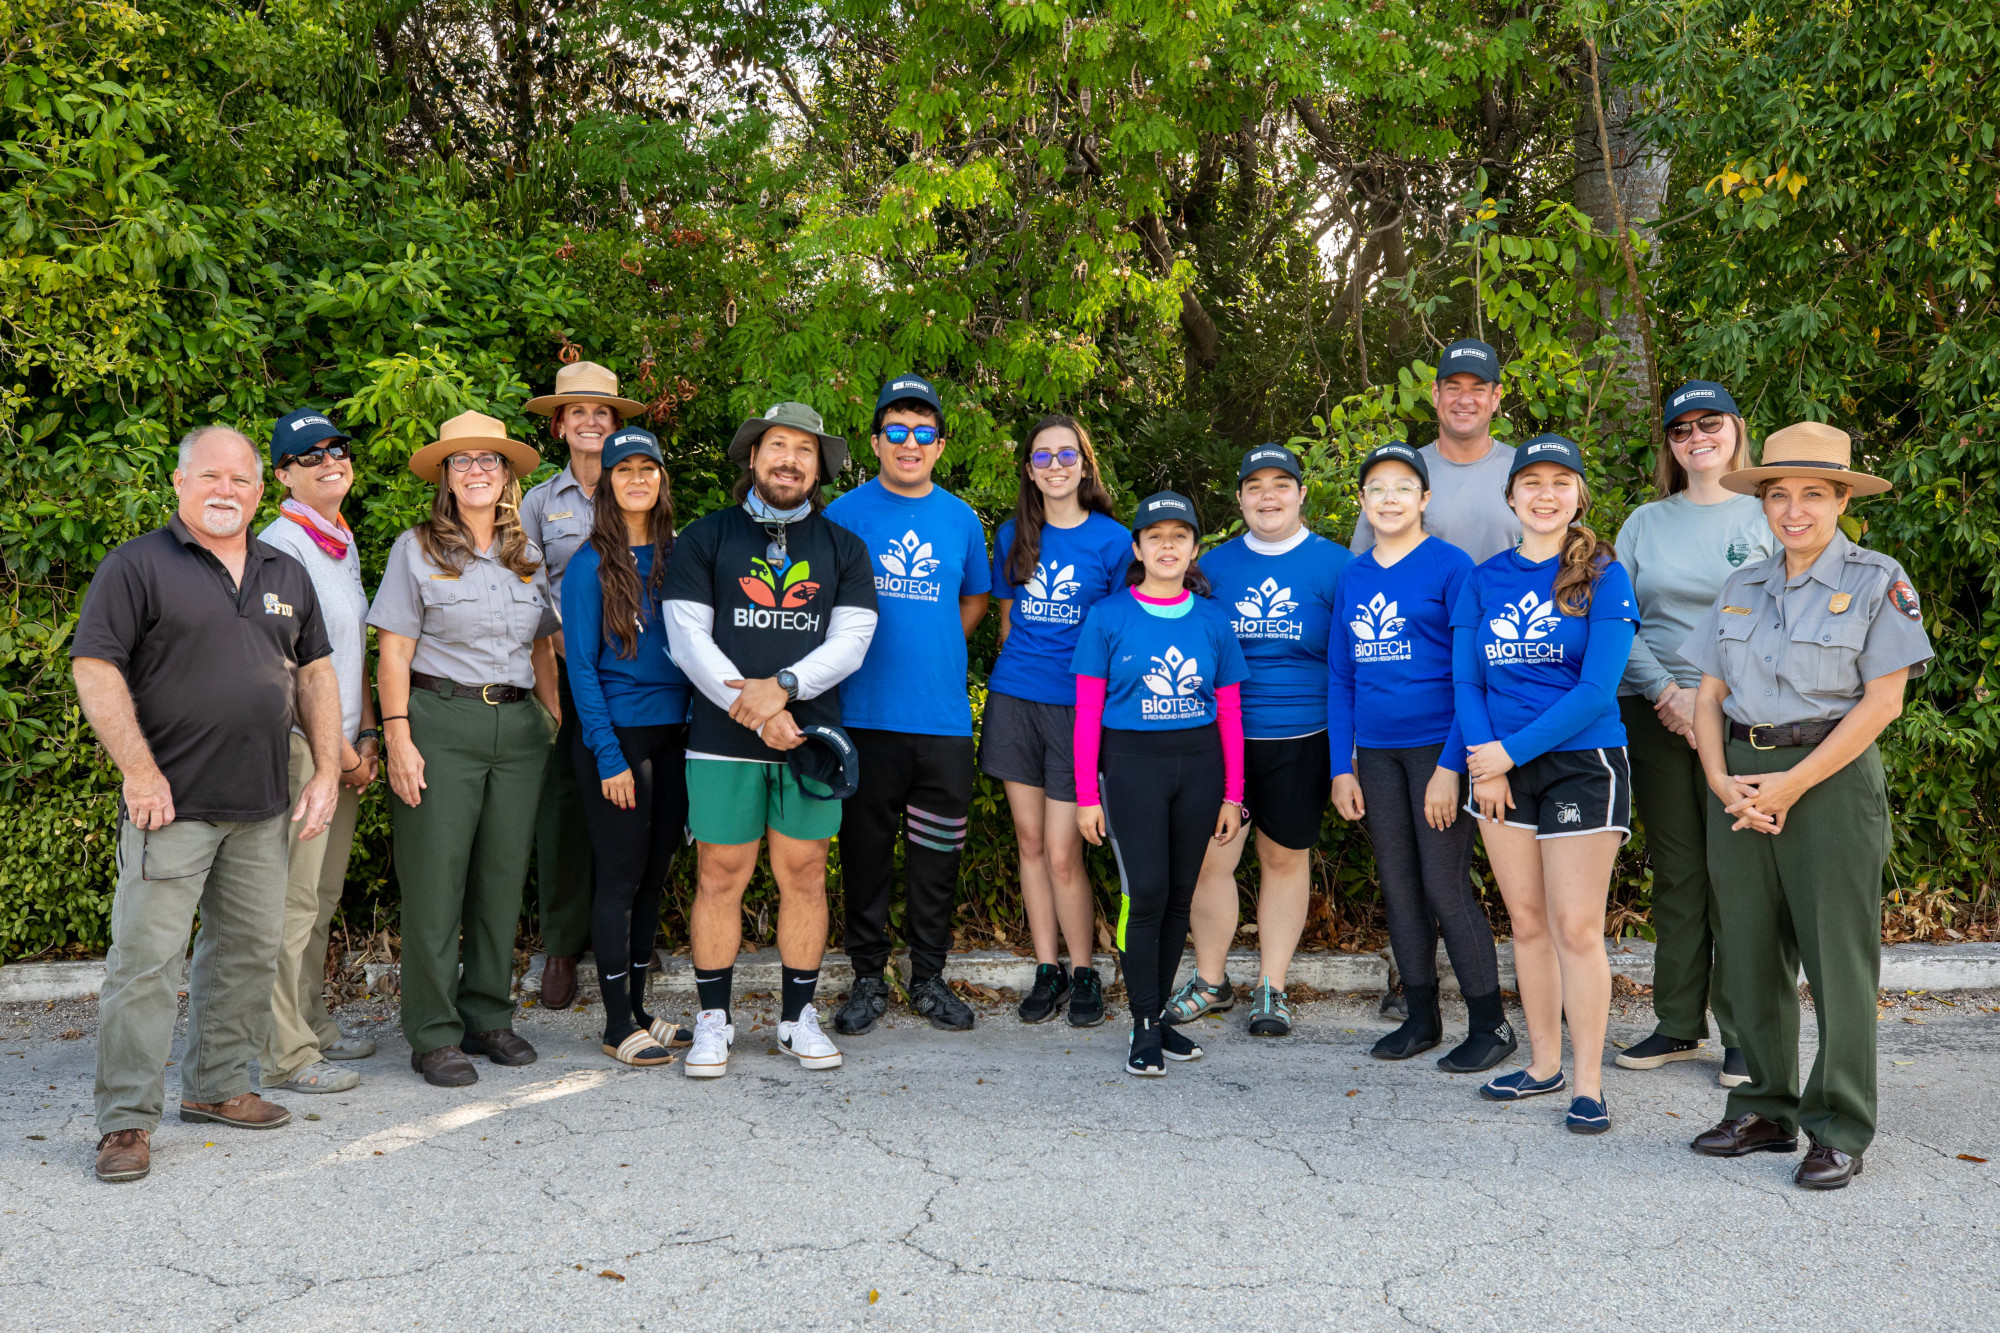
\includegraphics[width=\paperwidth]{images/23.jpg}}
%\end{center}%\maketitle

\maketitle

\section*{Highlights}

With 50\% of the samples analysed we can share the following highlights: \SI{17.5}{\litre} of water, roughly two buckets, contained:

\begin{itemize}
\item \textbf{12,458 unique sequences}
\item DNA from \textbf{163 identifiable species} of which 45 species were not previously reported in the Everglades. The Everglades is home to over 2,500 marine species (source UNESCO/Ocean Biodiversity Information System OBIS).
\item DNA of the following \textbf{threatened species}: Sphyrna tiburo (bonnethead shark, EN), Limulus polyphemus (horseshoe crab, VU), Negaprion brevirostris (lemon shark, VU), Trichechus manatus (West Indian manatee, VU), Megalops atlanticus (tarpon, VU), Epinephelus itajara (Atlantic goliath grouper, VU), Caretta caretta (logerhead sea turtle, VU).
\end{itemize}

\begin{figure}[h]
     \centering
     \begin{subfigure}[b]{0.48\textwidth}
         \centering
         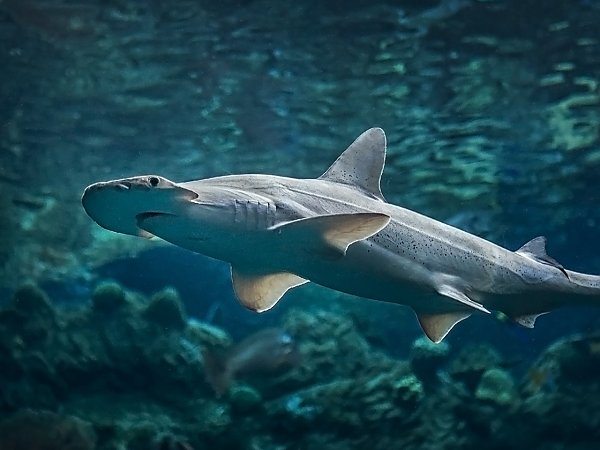
\includegraphics[width=\textwidth]{images/sphyrna_tiburo.jpg}
         \caption{Sphyrna tiburo}
     \end{subfigure}
     \hfill
     \begin{subfigure}[b]{0.48\textwidth}
         \centering
         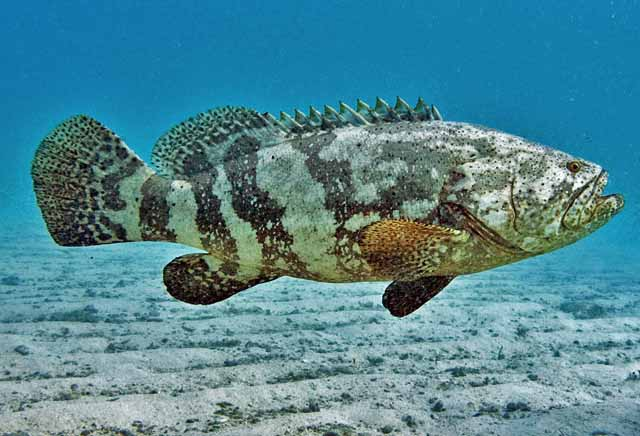
\includegraphics[width=\textwidth]{images/epinephelus_itajara.jpg}
         \caption{Epinephelus itajara}
     \end{subfigure}
     \hfill
     \begin{subfigure}[b]{0.48\textwidth}
         \centering
         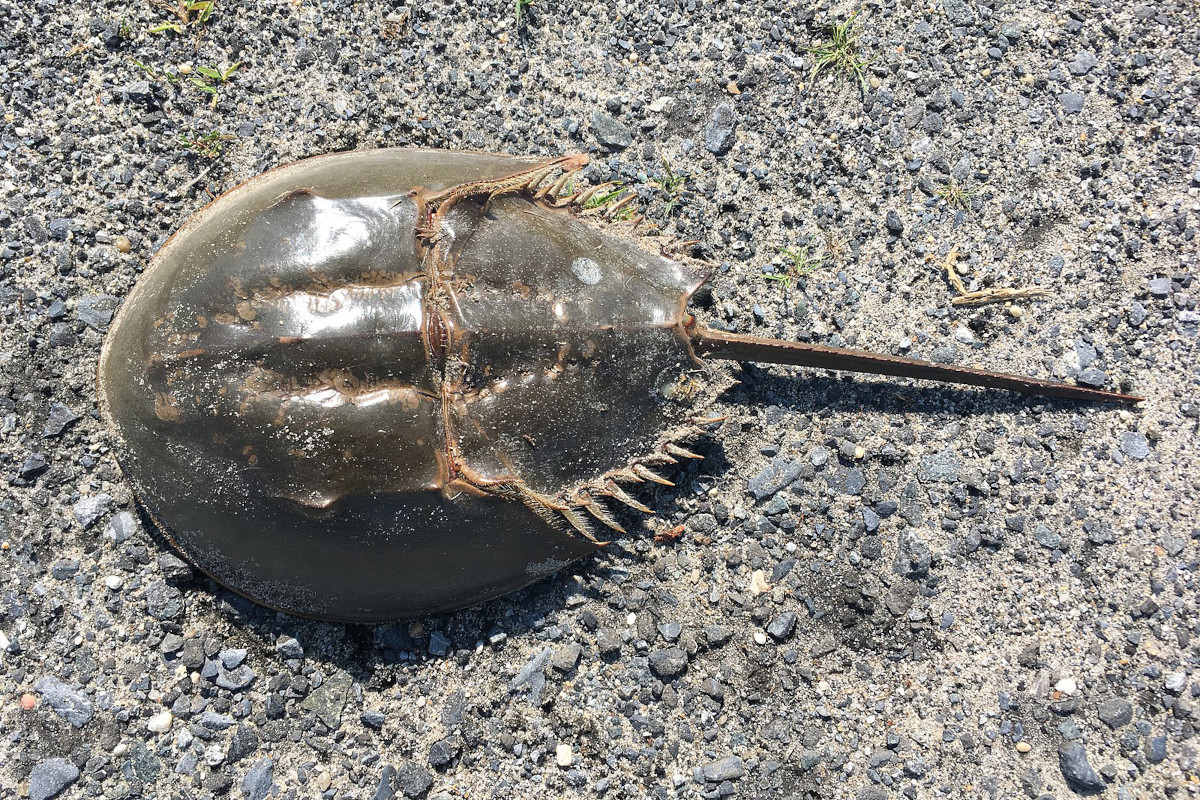
\includegraphics[width=\textwidth]{images/limulus_polyphemus.jpg}
         \caption{Limulus polyphemus}
     \end{subfigure}
     \hfill
     \begin{subfigure}[b]{0.48\textwidth}
         \centering
         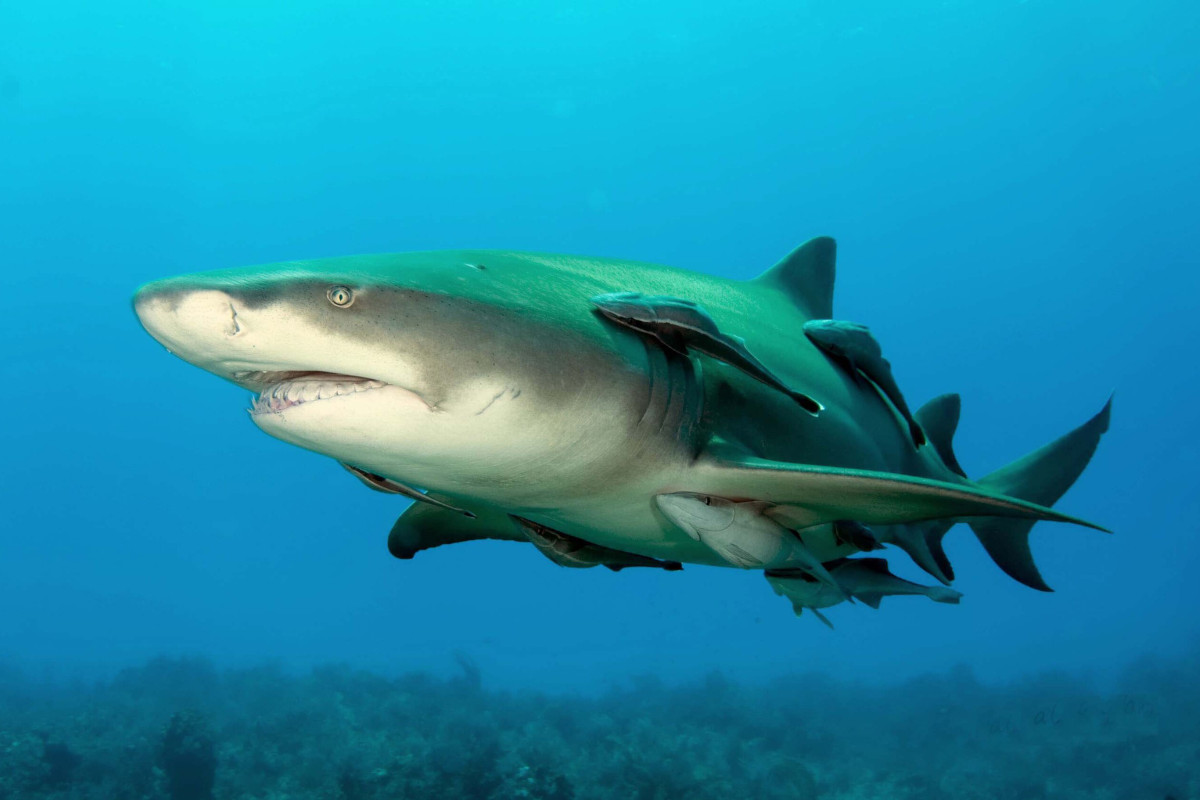
\includegraphics[width=\textwidth]{images/negaprion_brevirostris.jpg}
         \caption{Negaprion brevirostris}
     \end{subfigure}
     \hfill
     \begin{subfigure}[b]{0.48\textwidth}
         \centering
         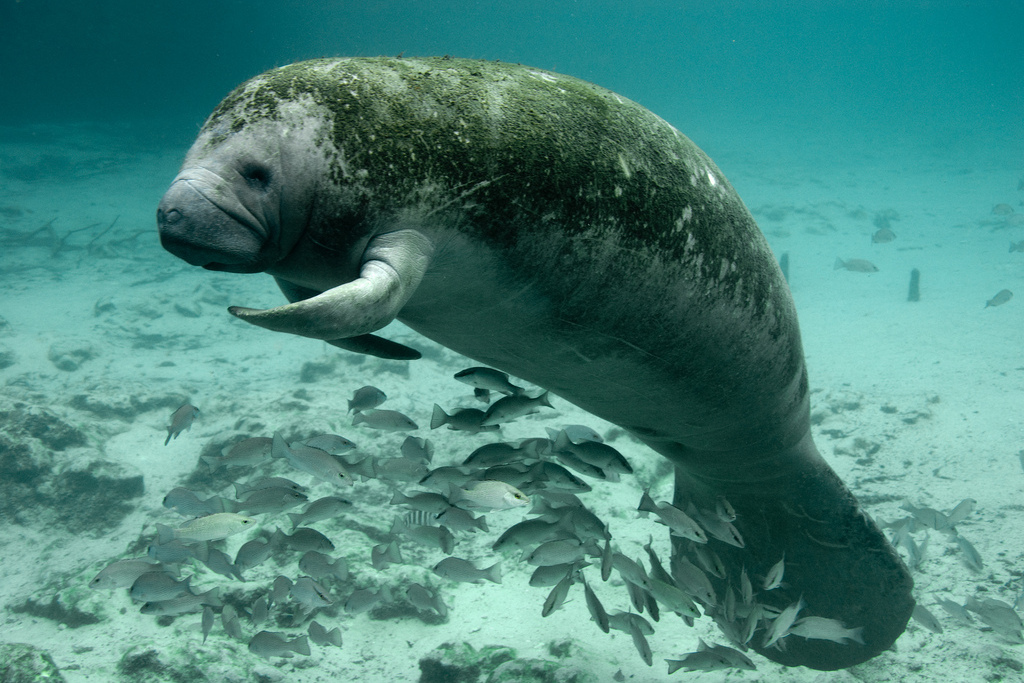
\includegraphics[width=\textwidth]{images/trichechus_manatus.jpg}
         \caption{Trichechus manatus}
     \end{subfigure}
     \hfill
     \begin{subfigure}[b]{0.48\textwidth}
         \centering
         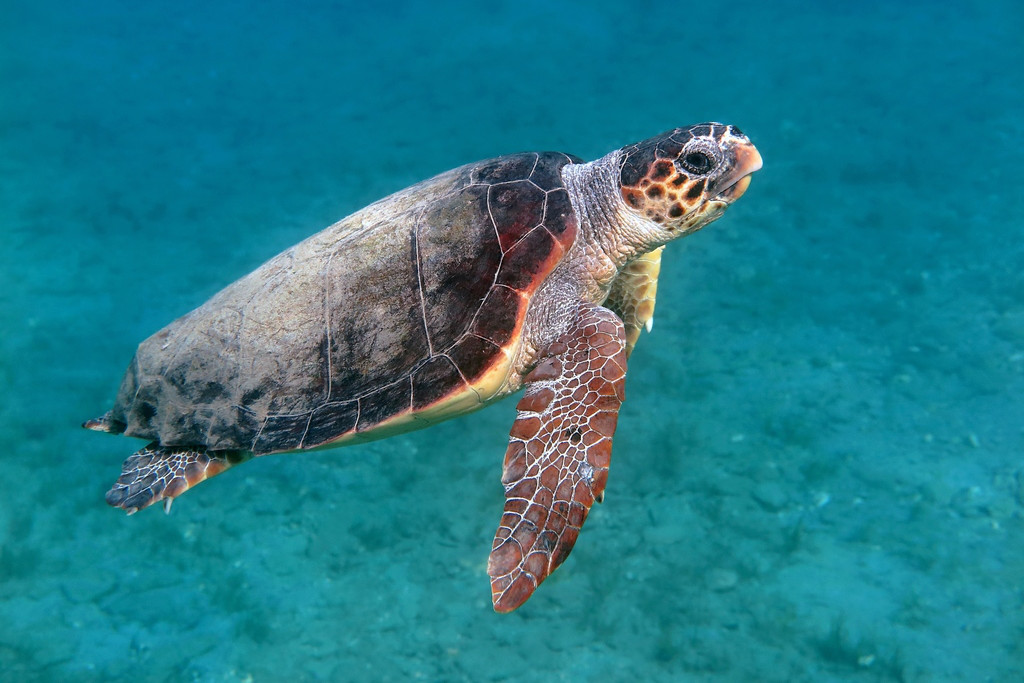
\includegraphics[width=\textwidth]{images/caretta_caretta.jpg}
         \caption{Caretta caretta}
     \end{subfigure}
     \caption{Some of the detected species. Credits: Robin Riggs (a), Smithsonian Tropical Research Institute (b), Albert Kok (d), U.S. Fish and Wildlife Service Headquarters (e), Roberto Pillon (f).}
\end{figure}

\clearpage

\section*{Introduction}

\begin{multicols}{2}
Environmental DNA Expeditions is a global, citizen science initiative that will help measure marine biodiversity, and the impacts climate change might have on the distribution patterns of marine life, across UNESCO World Heritage marine sites.

Ocean species shed DNA into the water around them. The genetic material from waste, mucus or cells in one liter of water can determine the species richness in a given area, without the need to actually extract organisms from their environment.
The cost effective, ethical nature of eDNA sampling has the potential to revolutionize knowledge about ecosystems and species diversity and to inspire the next generation of ocean researchers.
\end{multicols}

\begin{figure}[h]
\centering
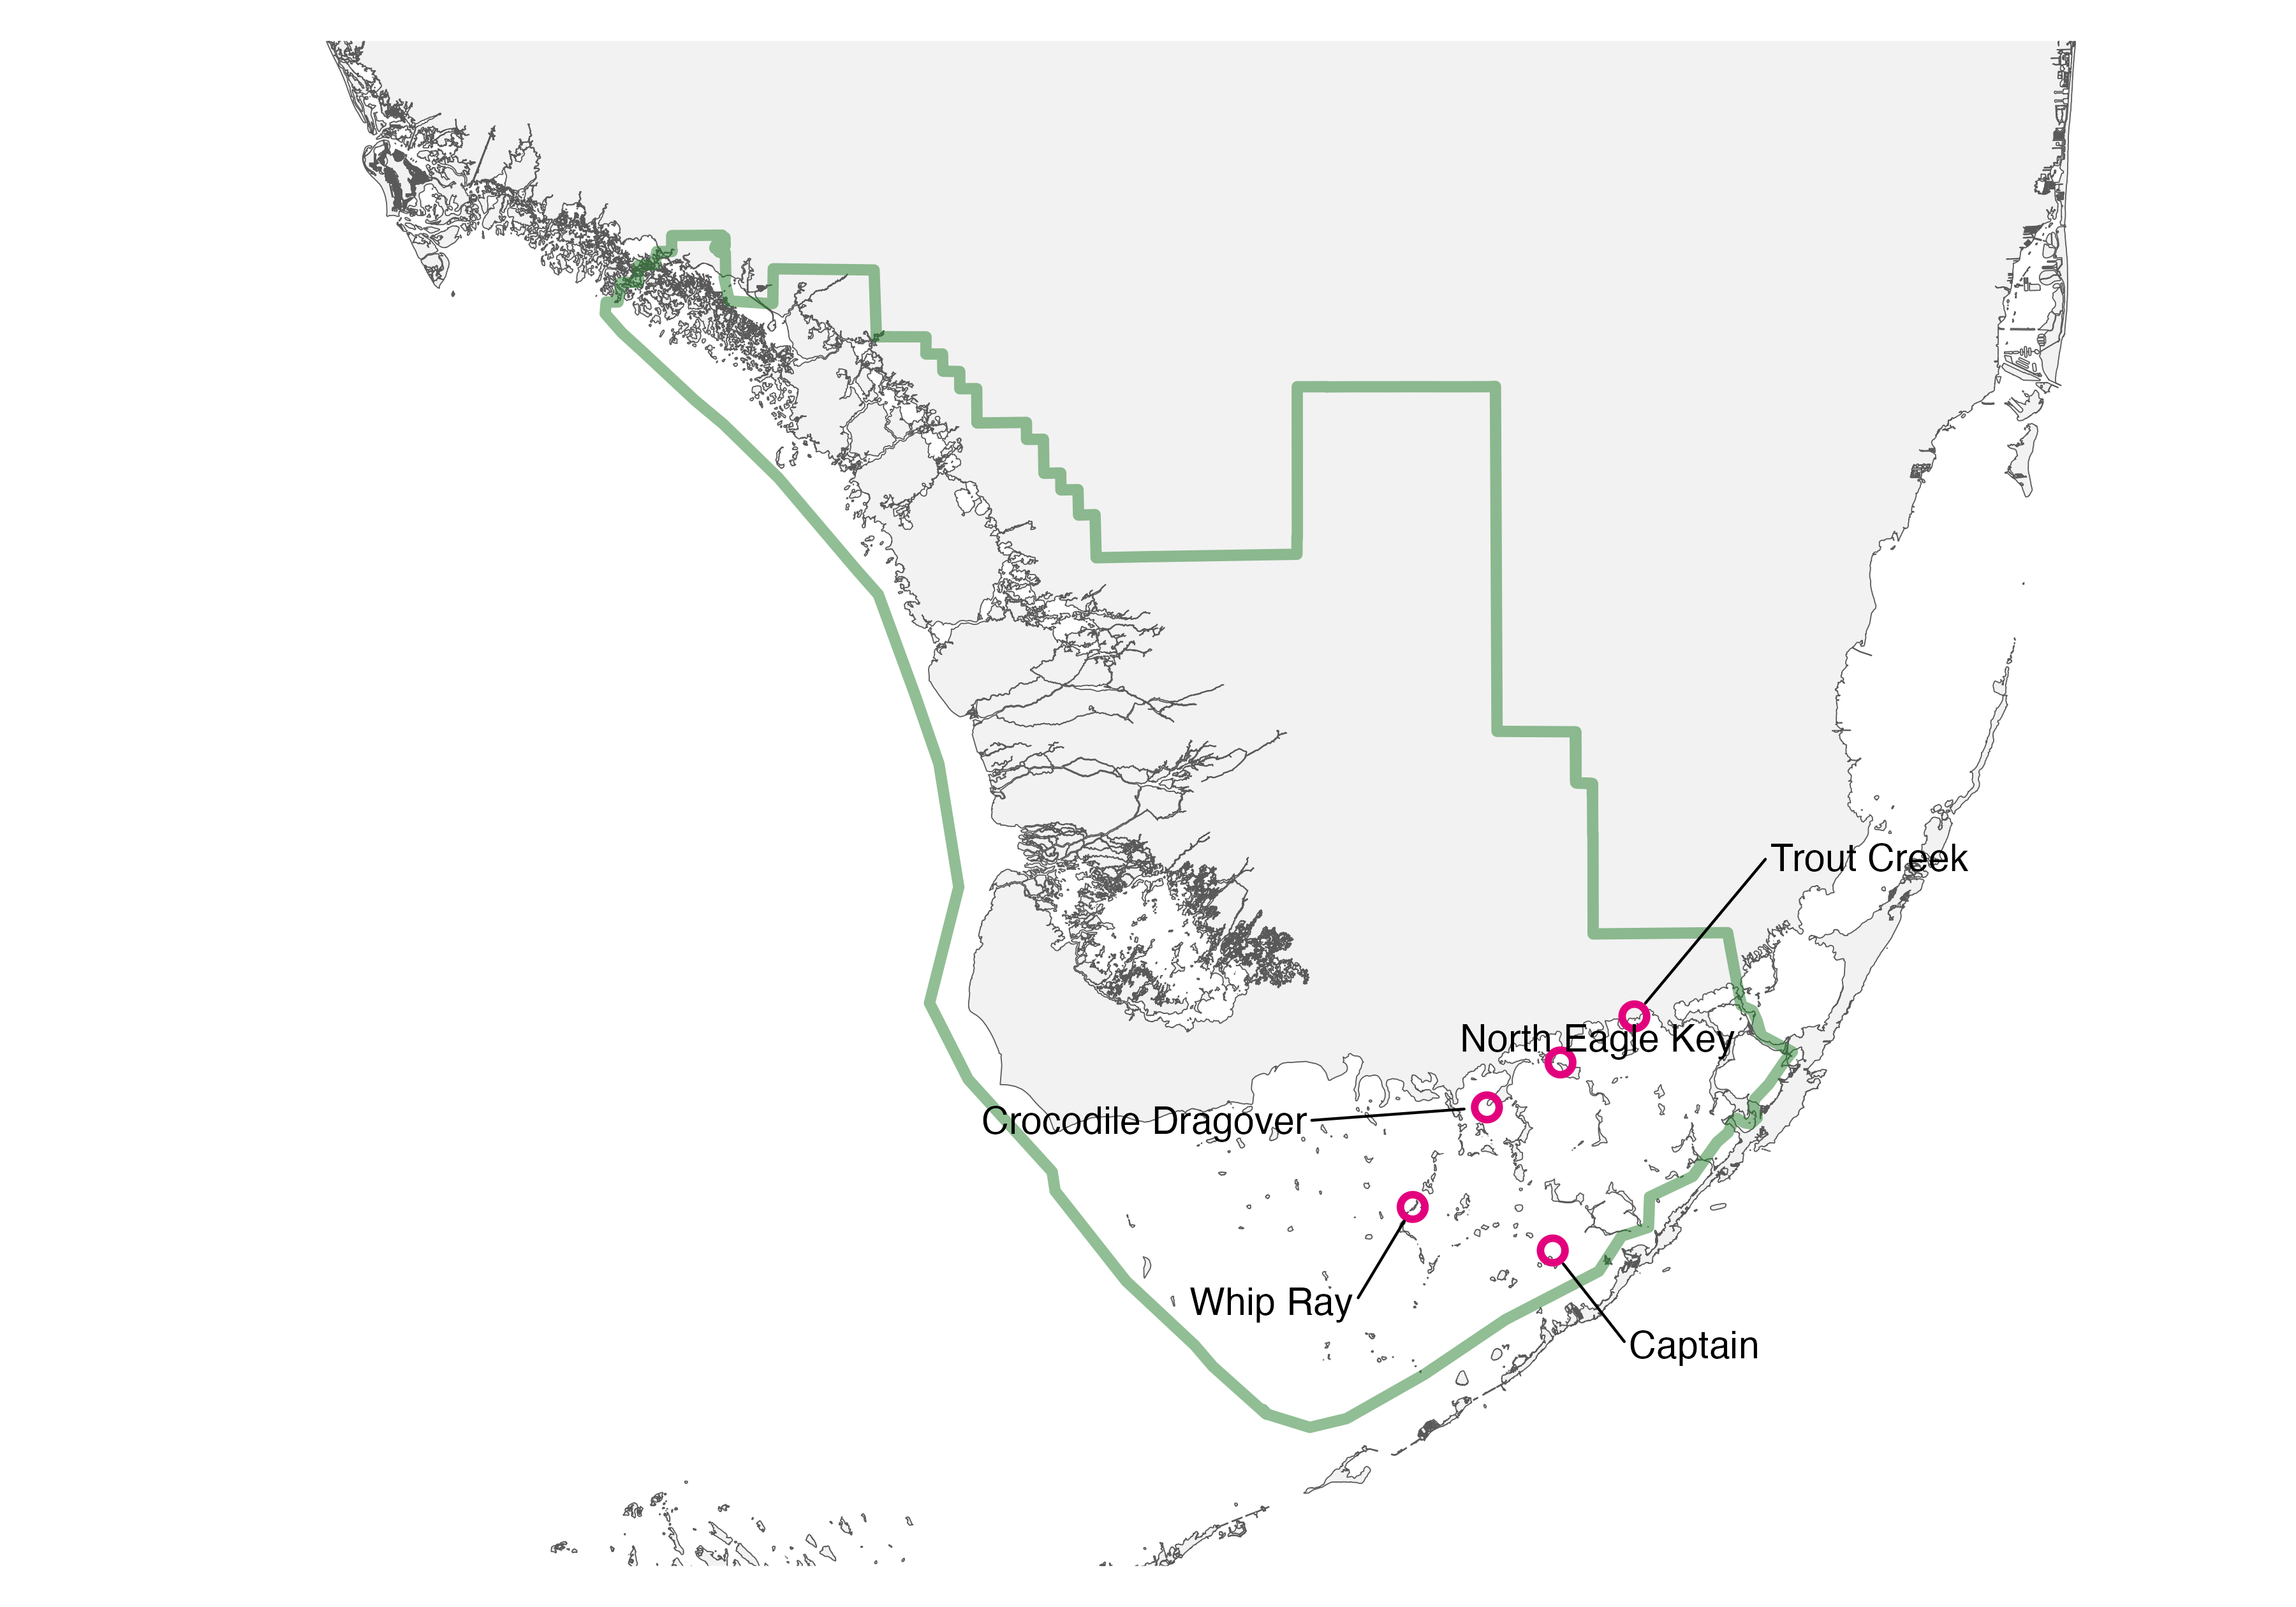
\includegraphics[width=\textwidth]{map}
\caption{Map of eDNA sampling locations}
\end{figure}

\section*{Results}
\subsection*{Sampling}

\begin{multicols}{2}
eDNA sampling was conducted in Everglades National Park in April 2023, by filtering up to \SI{1800}{\milli\litre} of seawater through filter cartridges with a \SI{0.8}{\micro\metre} pore size. 20 samples were collected at five locations in the park: Trout Creek, North Eagle Creek, Crocodile Dragover, Whip Ray, and Captain. From these 20 samples, a first batch of 11 samples covering all sites has been processed. DNA from these samples was extracted and amplified, and then sent to the sequencing facility.
\end{multicols}

\subsection*{DNA sequencing}

\begin{multicols}{2}
Sequencing of the DNA from 11 samples resulted in over 20 million sequence reads. From these reads we were able to collect 12,458 unique sequences or ASVs. Matching those sequences with reference sequences in public databases, we were able to detect 163 species. A total of 2,566 are known from Everglades National Park in the OBIS database. Of the 163 species detected, 45 are not known from the park in OBIS.
\end{multicols}

% latex table generated in R 4.2.2 by xtable 1.8-4 package
% Tue Nov 28 00:01:22 2023
\begin{longtable}{rrr}
  \hline
reads & species & asvs \\ 
  \hline
20543329 & 163 & 12458 \\ 
   \hline
\hline
\caption{Reads, ASVs, and species across all samples.} 
\label{table:stats}
\end{longtable}


% latex table generated in R 4.2.2 by xtable 1.8-4 package
% Mon Nov 27 11:07:42 2023
\begin{longtable}{llrrrr}
  \hline
locality & materialSampleID & reads & species & asvs & sampleSize \\ 
  \hline
Captain & EE0386 & 1715884 &  33 & 1630 & 1500 \\ 
  Captain & EE0391 & 1504564 &  77 & 6433 & 1800 \\ 
  Captain & EE0402 & 1768280 &  73 & 6949 & 1800 \\ 
  Crocodile Dragover & EE0389 & 1542386 &  64 & 6039 & 1500 \\ 
  Crocodile Dragover & EE0390 & 2070296 &  67 & 5909 & 450 \\ 
  North Eagle Key & EE0388 & 1586226 &  43 & 3460 & 1500 \\ 
  Trout Creek & EE0403 & 1854506 &  86 & 4358 & 1500 \\ 
  Whip Ray & EE0387 & 2902938 &  78 & 3966 & 1800 \\ 
  Whip Ray & EE0404 & 2195910 &  97 & 7002 & 1800 \\ 
  Whip Ray & EE0405 & 1994942 &  97 & 5646 & 1800 \\ 
  Whip Ray & EE0406 & 1491927 & 103 & 5601 & 1800 \\ 
   \hline
\hline
\end{longtable}


\clearpage

%\begin{figure}[h]
% 	\centering
% 	\makebox[\textwidth]{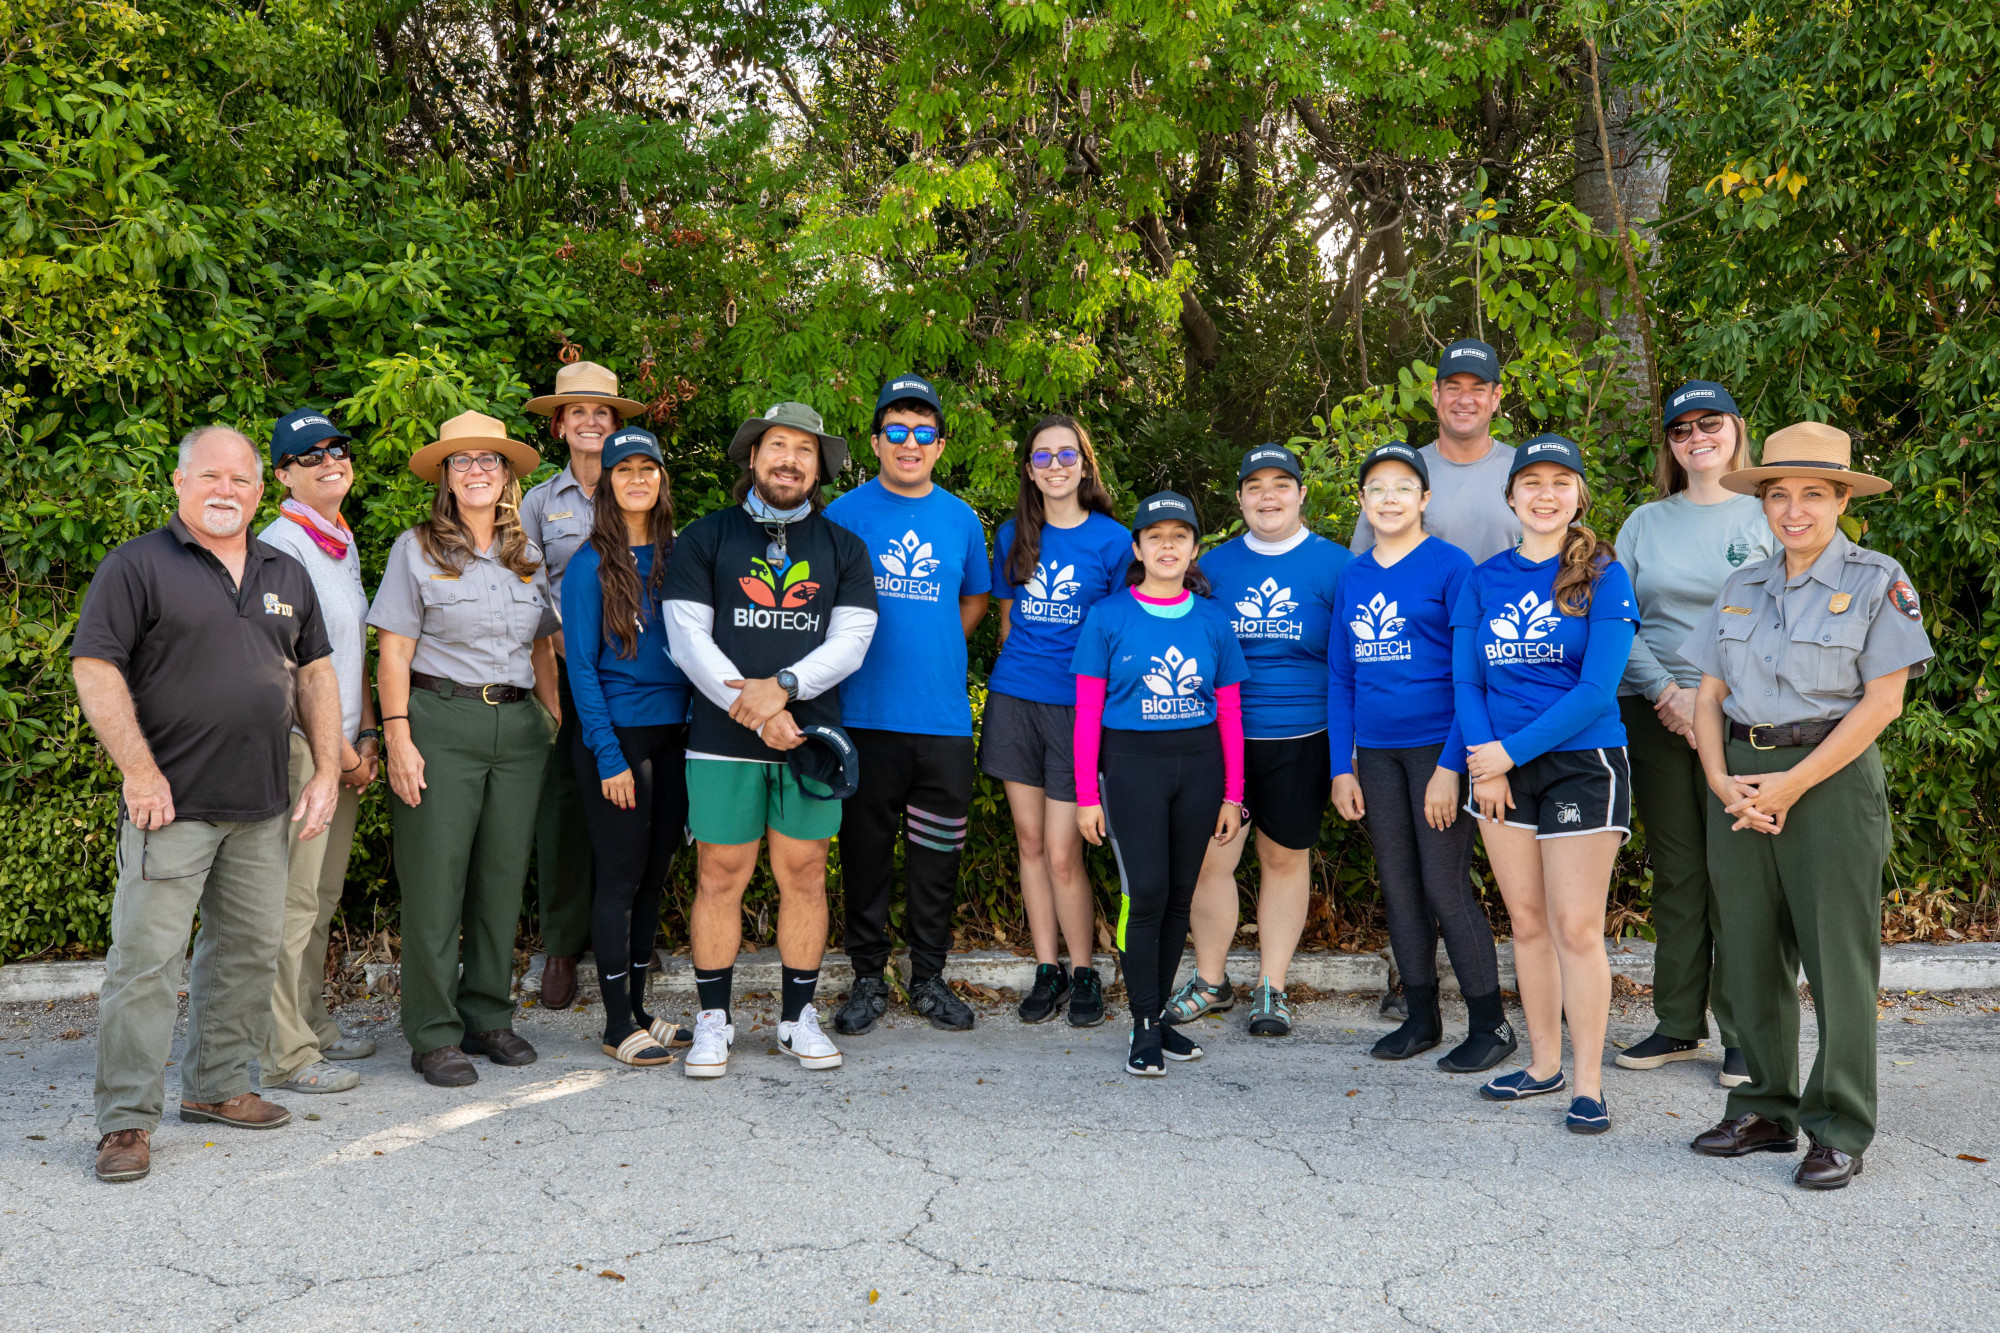
\includegraphics[width=0.6\paperwidth]{images/23.jpg}}
% 	\caption*{Credit: NPS Photos by Federico Acevedo}
%\end{figure}
%\begin{figure}[h]
% 	\centering
% 	\makebox[\textwidth]{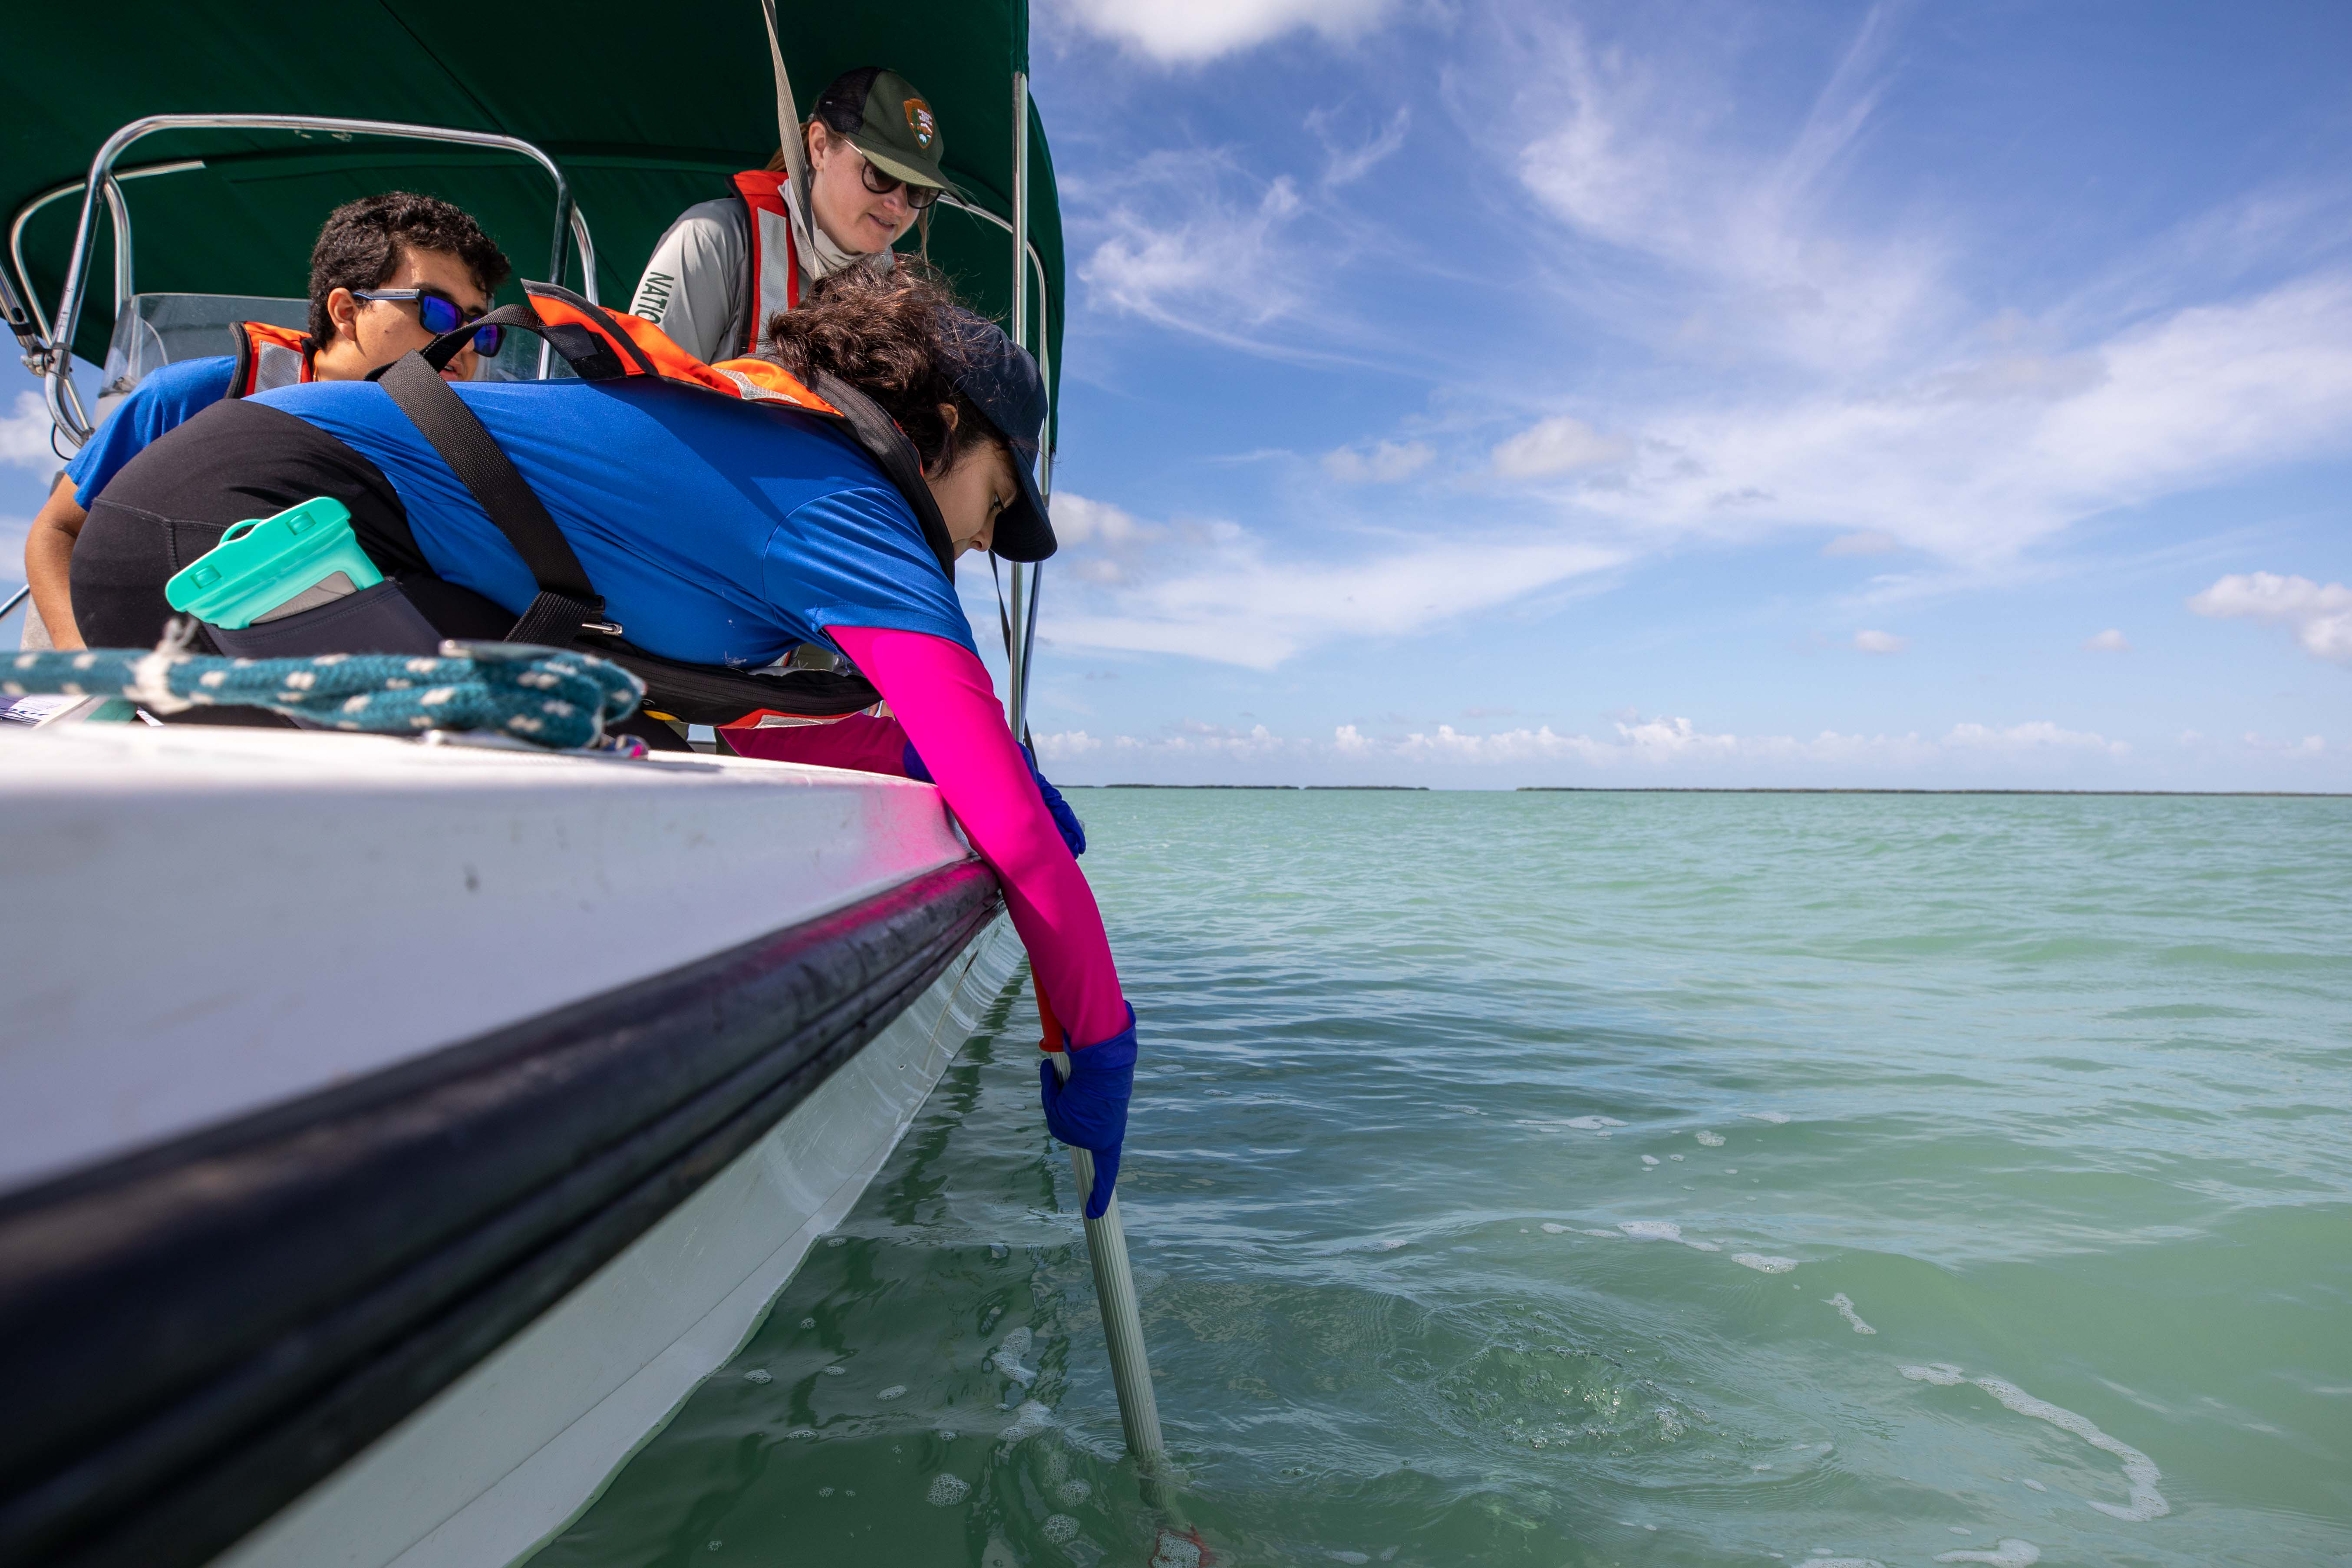
\includegraphics[width=0.6\paperwidth]{images/44.jpg}}
% 	\caption*{Credit: NPS Photos by Federico Acevedo}
%\end{figure}
%\begin{figure}[h]
% 	\centering
% 	\makebox[\textwidth]{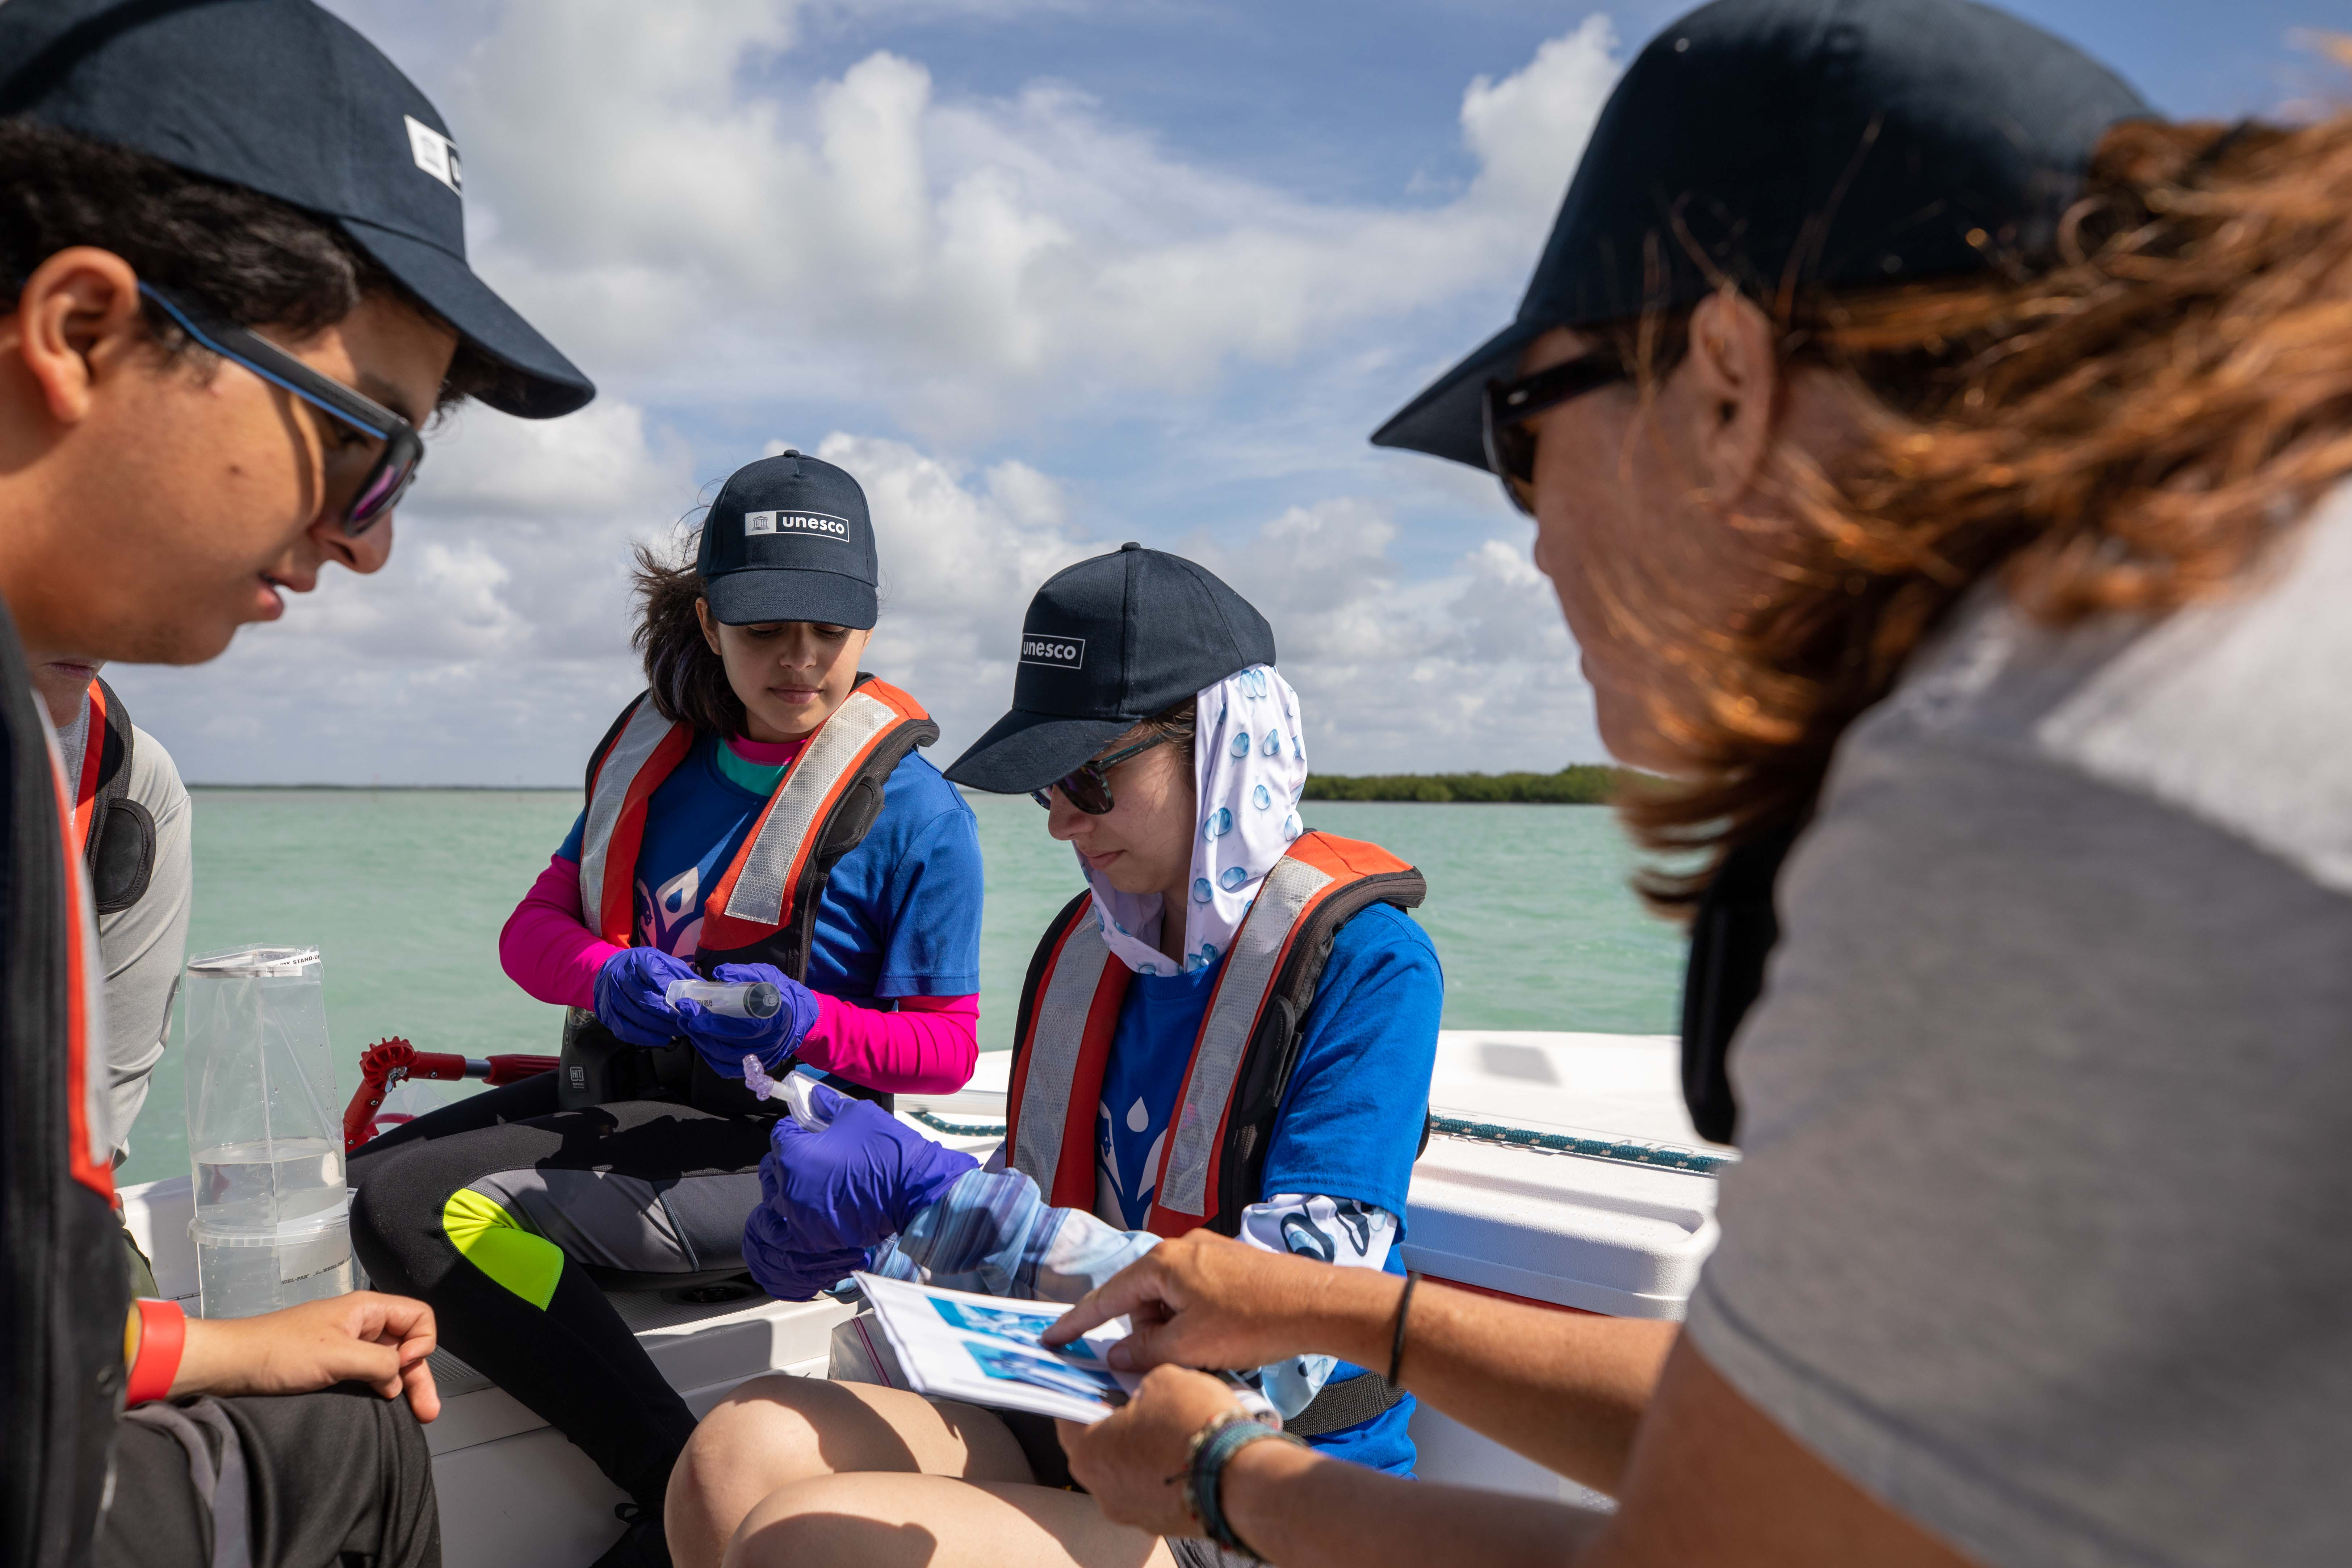
\includegraphics[width=0.6\paperwidth]{images/49.jpg}}
% 	\caption*{Credit: NPS Photos by Federico Acevedo}
%\end{figure}
%\begin{figure}[h]
% 	\centering
% 	\makebox[\textwidth]{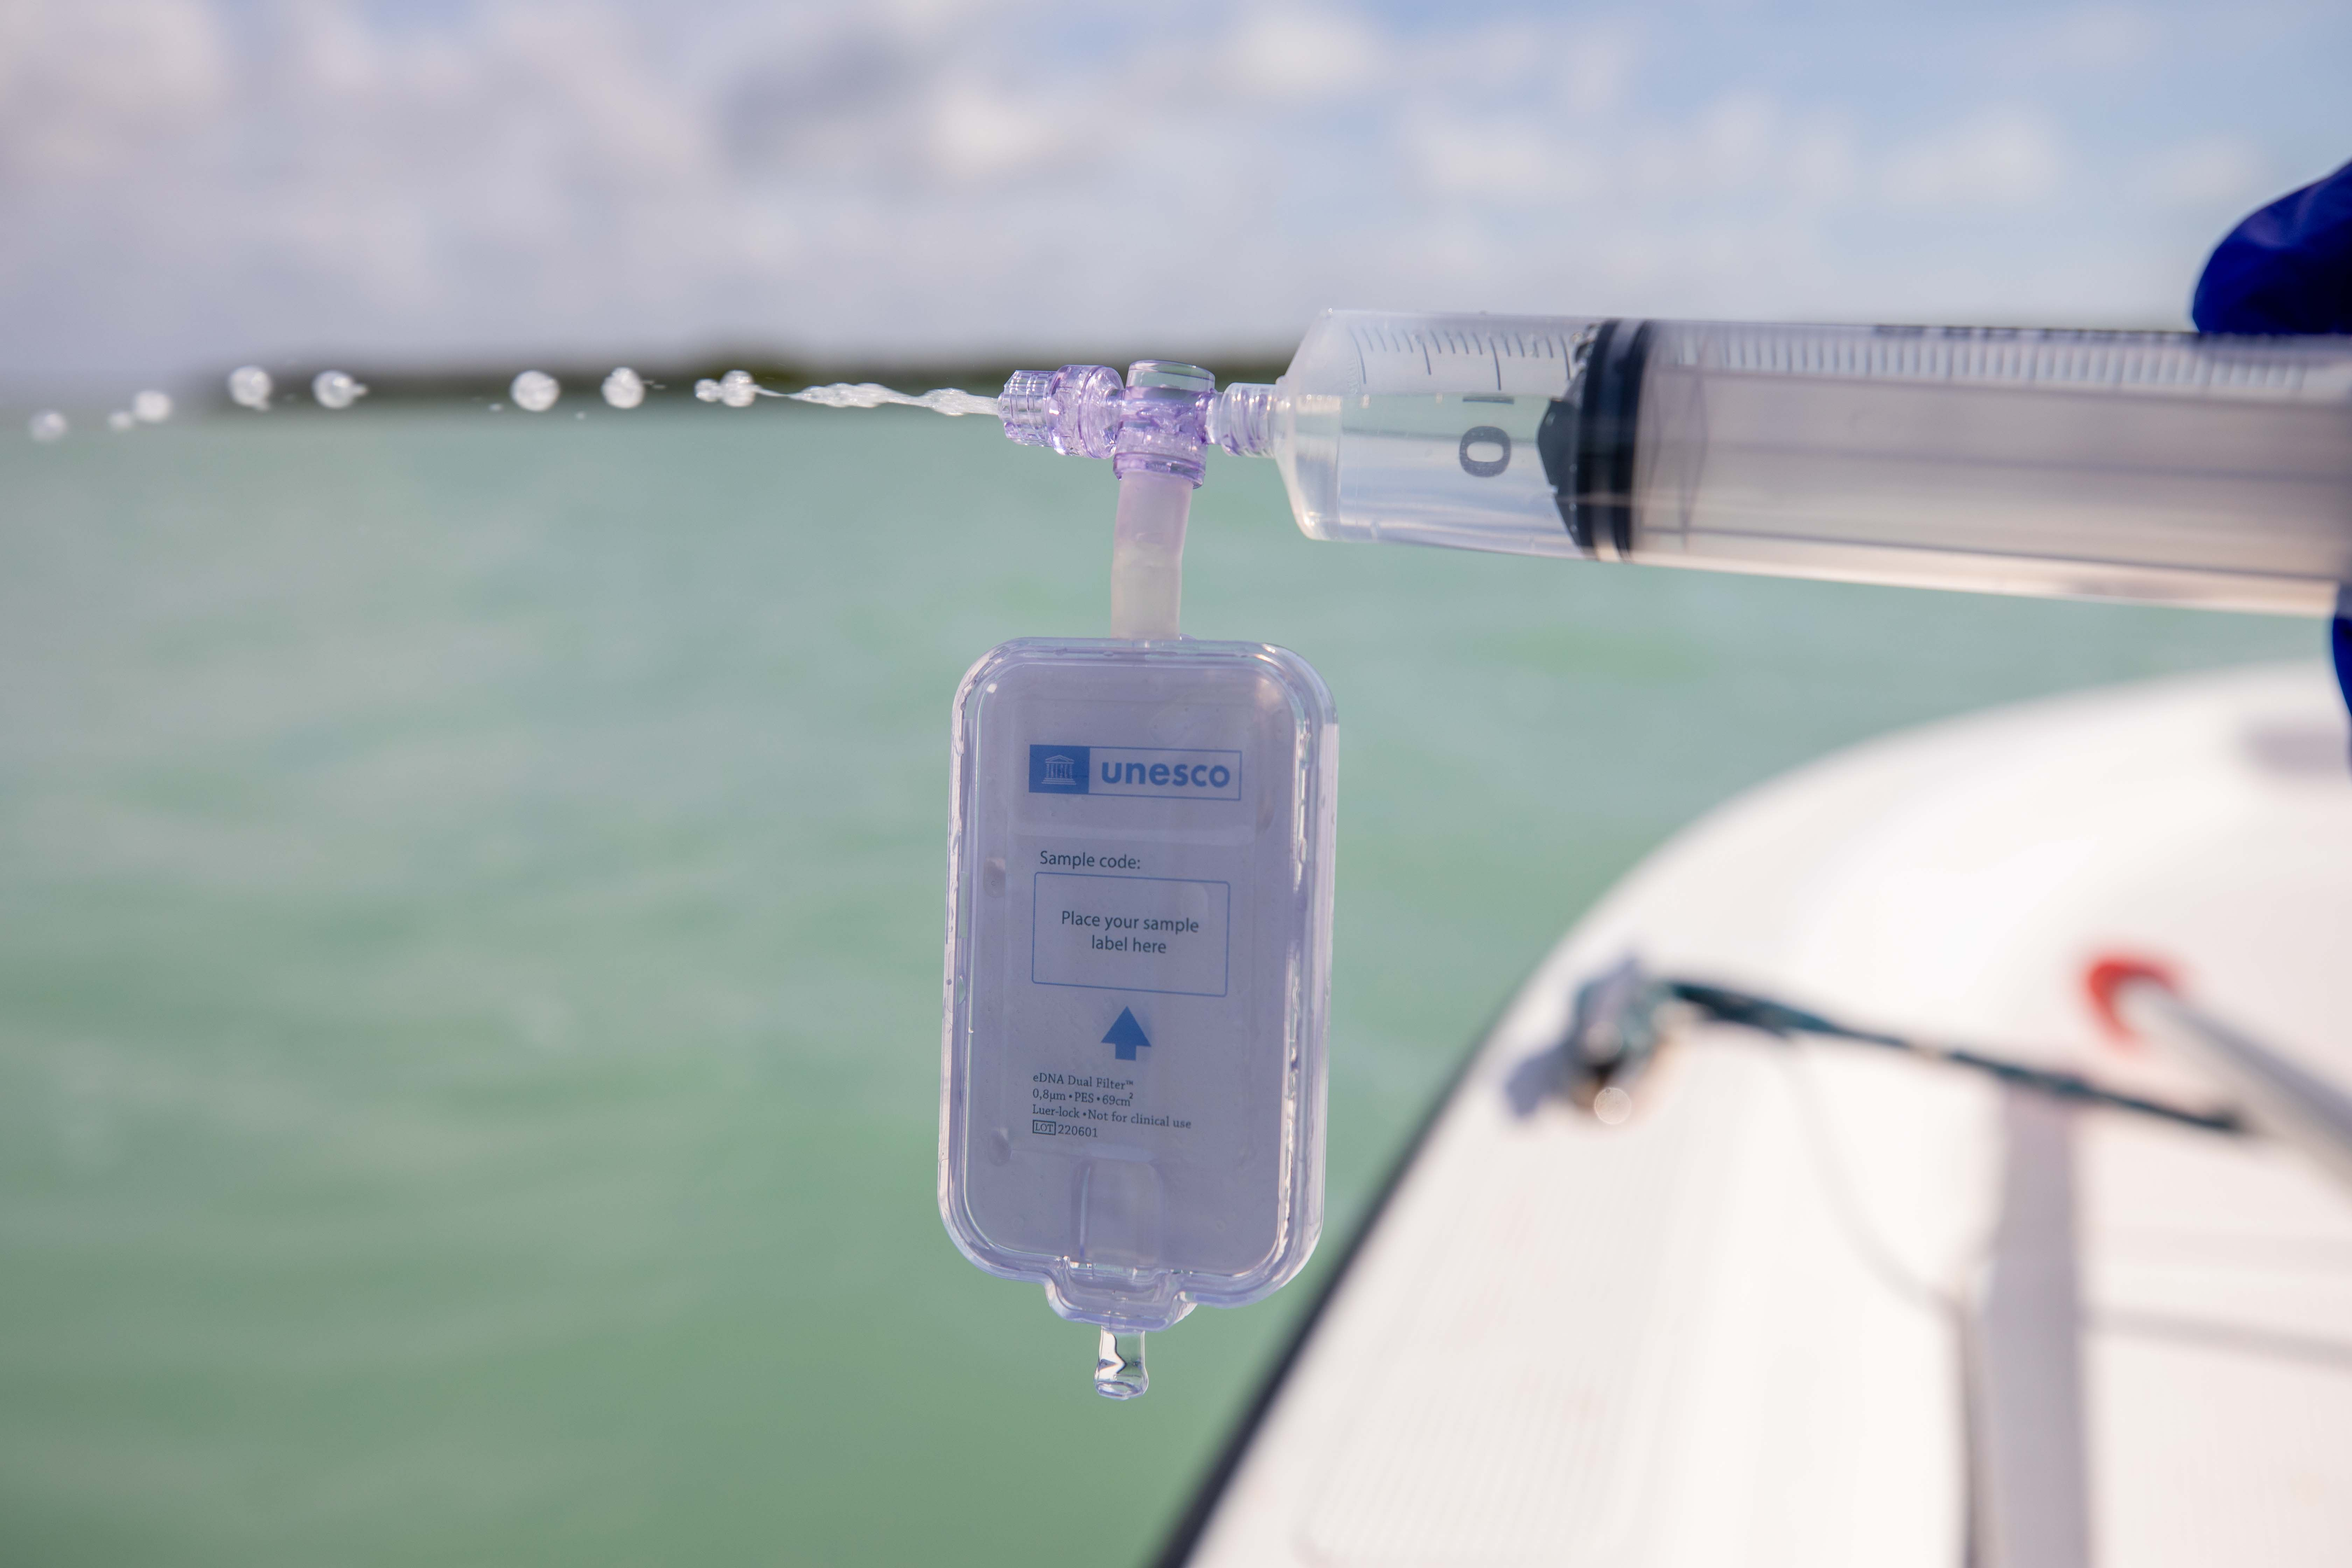
\includegraphics[width=0.6\paperwidth]{images/54.jpg}}
% 	\caption*{Credit: NPS Photos by Federico Acevedo}
%\end{figure}
%
%\clearpage

\begin{figure}[h!]
\centering
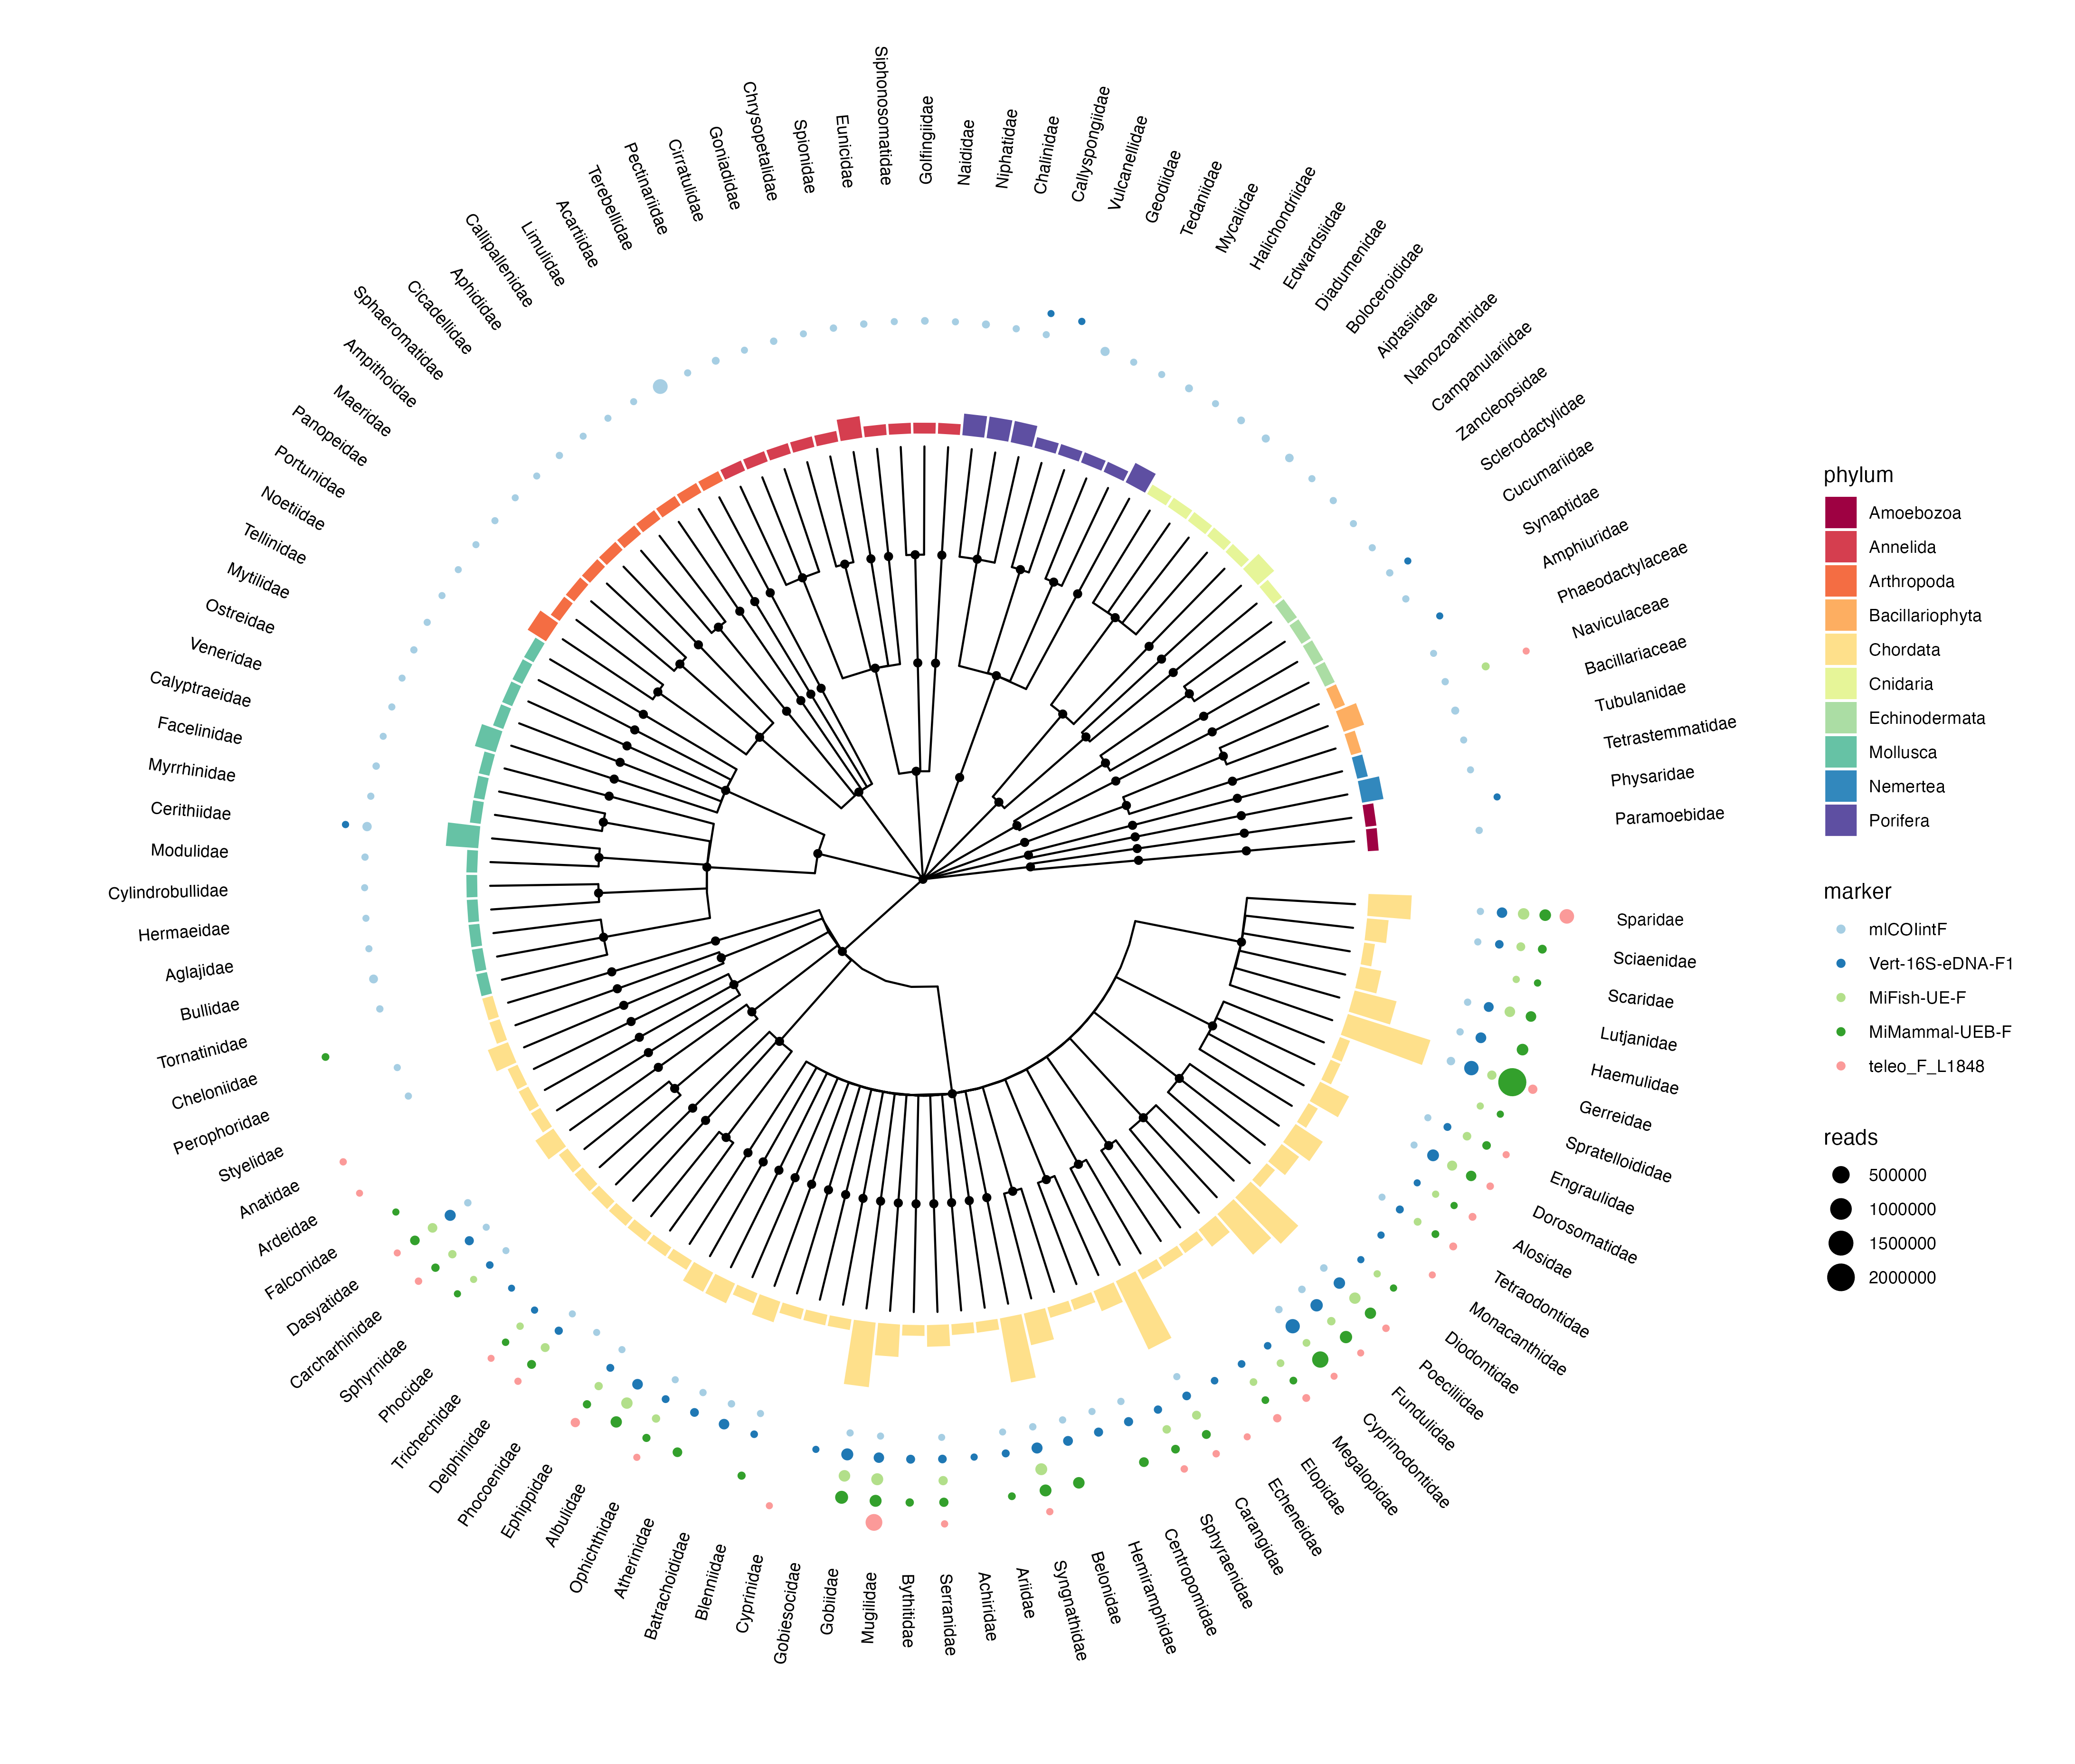
\includegraphics[width=\textwidth]{tree}
\caption{Number of DNA reads and species detected by family}
\end{figure}

\clearpage

\subsection*{Species identification}

\begin{multicols}{2}
The marker sequences obtained from sequencing were matched with sequence reference databases built using public data available from the National Center for Biotechnology Information (NCBI). This resulted in the identification of 163 species, of which 86 fish species, two mammalian species, and one turtle species. This represents about one sixth of the species known from Everglades National Park in the OBIS database. Seven of the detected species are listed as threatened on the IUCN Red List.
\end{multicols}

% latex table generated in R 4.2.2 by xtable 1.8-4 package
% Mon Nov 27 23:47:50 2023
\begin{longtable}{lrrr}
  \hline
group & obis\_species & edna\_species & fraction \\ 
  \hline
fish & 643 &  86 & 0.13 \\ 
  mammal &  13 &   2 & 0.15 \\ 
  turtle &   6 &   1 & 0.17 \\ 
   \hline
\hline
\caption{Number of species in the three target groups, from the OBIS database and from eDNA sampling.} 
\label{table:groups}
\end{longtable}


% latex table generated in R 4.2.2 by xtable 1.8-4 package
% Mon Nov 27 23:47:33 2023
\begin{longtable}{lrrr}
  \hline
category & obis\_species & edna\_species & fraction \\ 
  \hline
CR &  15 &  &  \\ 
  EN &  12 &   1 & 0.08 \\ 
  VU &  35 &   6 & 0.17 \\ 
   \hline
\hline
\caption{Number of species by IUCN Red List category, from the OBIS database and from eDNA sampling.} 
\label{table:categories}
\end{longtable}


\clearpage

\section*{Appendix: species list}

\begin{landscape}
% latex table generated in R 4.2.2 by xtable 1.8-4 package
% Thu Nov 30 10:52:34 2023
\begingroup\fontsize{9pt}{10pt}\selectfont
\begin{longtable}{lllllll}
  \hline
phylum & class & species & group & category & new & vernacular \\ 
  \hline 
\endhead 
\hline 
{\footnotesize Continued on next page} 
\endfoot 
\endlastfoot 
Amoebozoa & Discosea & Neoparamoeba aestuarina &  &  & yes &  \\ 
  Annelida & Clitellata & Thalassodrilides gurwitschi &  &  & yes &  \\ 
  Annelida & Polychaeta & Marphysa sanguinea &  &  &  & red rock worm \\ 
  Annelida & Polychaeta & Bhawania goodei &  &  & yes &  \\ 
  Annelida & Polychaeta & Glycinde multidens &  &  &  &  \\ 
  Annelida & Polychaeta & Polydora websteri &  &  & yes &  \\ 
  Annelida & Polychaeta & Prionospio steenstrupi &  &  &  &  \\ 
  Annelida & Polychaeta & Timarete caribous &  &  & yes &  \\ 
  Annelida & Polychaeta & Pectinaria gouldii &  &  &  & ice cream cone worm \\ 
  Annelida & Polychaeta & Loimia medusa &  &  &  & medusa worm \\ 
  Annelida &  & Golfingia (Golfingia) elongata &  &  &  &  \\ 
  Annelida &  & Siphonosoma cumanense &  &  & yes &  \\ 
  Arthropoda & Copepoda & Acartia (Acanthacartia) tonsa &  &  &  &  \\ 
  Arthropoda & Malacostraca & Cymadusa compta &  &  &  &  \\ 
  Arthropoda & Malacostraca & Neopanope packardii &  &  &  & Florida grassflat crab \\ 
  Arthropoda & Malacostraca & Callinectes sapidus &  &  &  & blue crab, crabe bleu \\ 
  Arthropoda & Malacostraca & Paracerceis caudata &  &  &  &  \\ 
  Arthropoda & Merostomata & Limulus polyphemus &  & VU &  & horseshoe crab \\ 
  Arthropoda & Pycnogonida & Callipallene brevirostris &  &  &  &  \\ 
  Bacillariophyta & Bacillariophyceae & Cylindrotheca closterium &  &  & yes &  \\ 
  Bacillariophyta & Bacillariophyceae & Haslea crucigera &  &  & yes &  \\ 
  Bacillariophyta & Bacillariophyceae & Navicula minima &  &  & yes &  \\ 
  Bacillariophyta & Bacillariophyceae & Phaeodactylum tricornutum &  &  & yes &  \\ 
  Bryozoa & Gymnolaemata & Amathia evelinae &  &  & yes &  \\ 
  Cercozoa & Chlorarachnea & Chlorarachnion reptans &  &  & yes &  \\ 
  Chlorophyta & Mamiellophyceae & Micromonas pusilla &  &  &  &  \\ 
  Chordata & Ascidiacea & Ecteinascidia styeloides &  &  & yes &  \\ 
  Chordata & Ascidiacea & Botrylloides niger &  &  &  & Black synascidia , Synascidie noire \\ 
  Chordata & Aves & Falco sparverius &  & LC & yes &  \\ 
  Chordata & Elasmobranchii & Negaprion brevirostris & fish & VU &  & lemon shark \\ 
  Chordata & Elasmobranchii & Sphyrna tiburo & fish & EN &  & bonnethead \\ 
  Chordata & Elasmobranchii & Hypanus americanus & fish & NT &  &  \\ 
  Chordata & Mammalia & Tursiops truncatus & mammal & LC &  & bottlenose dolphin, grand dauphin \\ 
  Chordata & Mammalia & Trichechus manatus & mammal & VU &  & West Indian manatee \\ 
  Chordata & Teleostei & Chaetodipterus faber & fish & LC &  & Atlantic spadefish \\ 
  Chordata & Teleostei & Albula vulpes & fish & NT &  & bonefish \\ 
  Chordata & Teleostei & Myrophis punctatus & fish & LC &  & speckled worm eel \\ 
  Chordata & Teleostei & Atherinomorus stipes & fish & LC &  & hardhead silverside \\ 
  Chordata & Teleostei & Opsanus beta & fish & LC &  & Gulf toadfish \\ 
  Chordata & Teleostei & Opsanus tau & fish & LC &  & oyster toadfish \\ 
  Chordata & Teleostei & Strongylura notata & fish & LC &  & redfin needlefish \\ 
  Chordata & Teleostei & Strongylura timucu & fish & LC &  & timucu \\ 
  Chordata & Teleostei & Tylosurus crocodilus & fish & LC &  & houndfish \\ 
  Chordata & Teleostei & Chriodorus atherinoides & fish & LC &  & hardhead halfbeak \\ 
  Chordata & Teleostei & Chasmodes bosquianus & fish & LC &  & striped blenny \\ 
  Chordata & Teleostei & Centropomus undecimalis & fish & LC &  & common snook \\ 
  Chordata & Teleostei & Sphyraena barracuda & fish & LC &  & great barracuda \\ 
  Chordata & Teleostei & Caranx crysos & fish & LC &  & blue runner, carangue coubali \\ 
  Chordata & Teleostei & Caranx hippos & fish & LC &  & common jack, carangue crevalle \\ 
  Chordata & Teleostei & Caranx latus & fish & LC &  & horse-eye jack \\ 
  Chordata & Teleostei & Oligoplites saurus & fish & LC &  & leatherjack \\ 
  Chordata & Teleostei & Selene vomer & fish & LC &  & lookdown \\ 
  Chordata & Teleostei & Trachinotus carolinus & fish & LC &  & pompano \\ 
  Chordata & Teleostei & Echeneis naucrates & fish & LC &  & sharksucker \\ 
  Chordata & Teleostei & Brevoortia patronus & fish & LC &  & Gulf menhaden \\ 
  Chordata & Teleostei & Harengula jaguana & fish & LC &  & scaled sardine \\ 
  Chordata & Teleostei & Opisthonema oglinum & fish & LC &  & Atlantic thread herring \\ 
  Chordata & Teleostei & Anchoa mitchilli & fish & LC &  & bay anchovy \\ 
  Chordata & Teleostei & Jenkinsia lamprotaenia & fish & LC &  & dwarf herring \\ 
  Chordata & Teleostei & Cyprinodon variegatus & fish & LC &  & sheepshead minnow \\ 
  Chordata & Teleostei & Floridichthys carpio & fish & LC &  & goldspotted killifish \\ 
  Chordata & Teleostei & Fundulus confluentus & fish & LC &  & marsh killifish \\ 
  Chordata & Teleostei & Fundulus grandis & fish & LC &  & Gulf killifish \\ 
  Chordata & Teleostei & Fundulus xenicus & fish &  &  &  \\ 
  Chordata & Teleostei & Lucania goodei & fish & LC & yes &  \\ 
  Chordata & Teleostei & Lucania parva & fish & LC &  & rainwater killifish \\ 
  Chordata & Teleostei & Belonesox belizanus & fish & LC &  & pike killifish \\ 
  Chordata & Teleostei & Gambusia affinis & fish & LC &  & mosquitofish \\ 
  Chordata & Teleostei & Gambusia holbrooki & fish & LC &  & eastern mosquitofish \\ 
  Chordata & Teleostei & Gambusia rhizophorae & fish & LC &  & mangrove gambusia \\ 
  Chordata & Teleostei & Poecilia latipinna & fish & LC &  & sailfin molly \\ 
  Chordata & Teleostei & Poecilia sphenops & fish & LC & yes & Mexican molly \\ 
  Chordata & Teleostei & Elops saurus & fish & LC &  & ladyfish \\ 
  Chordata & Teleostei & Megalops atlanticus & fish & VU &  & tarpon \\ 
  Chordata & Teleostei & Diapterus auratus & fish & LC &  & Irish mojarra \\ 
  Chordata & Teleostei & Eucinostomus argenteus & fish & LC &  & silver mojarra \\ 
  Chordata & Teleostei & Eucinostomus gula & fish & LC &  & Jenny mojarra \\ 
  Chordata & Teleostei & Eucinostomus jonesii & fish & LC &  & slender mojarra \\ 
  Chordata & Teleostei & Eucinostomus melanopterus & fish & LC &  & flagfin mojarra \\ 
  Chordata & Teleostei & Eugerres plumieri & fish & LC &  & striped mojarra \\ 
  Chordata & Teleostei & Gerres cinereus & fish & LC &  & yellowfin mojarra \\ 
  Chordata & Teleostei & Ulaema lefroyi & fish &  &  &  \\ 
  Chordata & Teleostei & Haemulon aurolineatum & fish & LC &  & tomtate grunt \\ 
  Chordata & Teleostei & Haemulon parra & fish & LC &  & sailors choice \\ 
  Chordata & Teleostei & Haemulon plumierii & fish & LC &  & grunt \\ 
  Chordata & Teleostei & Haemulon sciurus & fish & LC &  & bluestriped grunt \\ 
  Chordata & Teleostei & Lutjanus griseus & fish & LC &  & grey snapper \\ 
  Chordata & Teleostei & Nicholsina usta & fish & LC &  & emerald parrotfish \\ 
  Chordata & Teleostei & Cynoscion nebulosus & fish & LC &  & spotted weakfish \\ 
  Chordata & Teleostei & Pogonias cromis & fish & LC &  & blackdrum \\ 
  Chordata & Teleostei & Archosargus probatocephalus & fish & LC &  & sheepshead \\ 
  Chordata & Teleostei & Archosargus rhomboidalis & fish & LC &  & Western Atlantic seabream \\ 
  Chordata & Teleostei & Diplodus holbrookii & fish & LC &  & spottail pinfish \\ 
  Chordata & Teleostei & Lagodon rhomboides & fish & LC &  & pinfish \\ 
  Chordata & Teleostei & Gobiesox strumosus & fish & LC &  & skilletfish \\ 
  Chordata & Teleostei & Gobiosoma bosc & fish & LC &  & naked goby \\ 
  Chordata & Teleostei & Gobiosoma robustum & fish & LC &  & code goby \\ 
  Chordata & Teleostei & Lophogobius cyprinoides & fish & LC &  & crested goby \\ 
  Chordata & Teleostei & Microgobius gulosus & fish & LC &  & clown goby \\ 
  Chordata & Teleostei & Microgobius microlepis & fish & LC &  & banner goby \\ 
  Chordata & Teleostei & Mugil cephalus & fish & LC &  & grey mullet, muge \\ 
  Chordata & Teleostei & Mugil curema & fish & LC &  & silverside mullet \\ 
  Chordata & Teleostei & Mugil rubrioculus & fish & LC &  &  \\ 
  Chordata & Teleostei & Ogilbia cayorum & fish & LC &  & key brotula \\ 
  Chordata & Teleostei & Epinephelus itajara & fish & VU &  & itajara \\ 
  Chordata & Teleostei & Trinectes maculatus & fish & LC &  & hogchoker \\ 
  Chordata & Teleostei & Ariopsis felis & fish & LC &  & hardhead catfish \\ 
  Chordata & Teleostei & Anarchopterus criniger & fish & LC &  & fringed pipefish \\ 
  Chordata & Teleostei & Hippocampus zosterae & fish & LC &  & dwarf seahorse \\ 
  Chordata & Teleostei & Syngnathus floridae & fish & LC &  & dusky pipefish \\ 
  Chordata & Teleostei & Syngnathus fuscus & fish & LC &  & northern pipefish \\ 
  Chordata & Teleostei & Syngnathus schlegeli & fish & LC & yes & Seaweed pipefish \\ 
  Chordata & Teleostei & Chilomycterus schoepfii & fish & LC &  & striped burrfish \\ 
  Chordata & Teleostei & Stephanolepis hispida & fish &  &  &  \\ 
  Chordata & Teleostei & Sphoeroides maculatus & fish & LC &  & puffer \\ 
  Chordata & Teleostei & Sphoeroides parvus & fish & LC & yes & least puffer \\ 
  Chordata & Teleostei & Sphoeroides spengleri & fish & LC &  & bandtail puffer \\ 
  Chordata &  & Caretta caretta & turtle & VU &  & logerhead sea turtle, tortue Caouanne \\ 
  Cnidaria & Anthozoa & Exaiptasia diaphana &  &  &  &  \\ 
  Cnidaria & Anthozoa & Boloceroides mcmurrichi &  &  & yes &  \\ 
  Cnidaria & Anthozoa & Diadumene leucolena &  &  & yes & white anemone \\ 
  Cnidaria & Anthozoa & Nanozoanthus harenaceus &  &  & yes &  \\ 
  Cnidaria & Hydrozoa & Zancleopsis dichotoma &  &  & yes &  \\ 
  Cnidaria & Hydrozoa & Clytia hemisphaerica &  &  & yes &  \\ 
  Cnidaria & Hydrozoa & Obelia bidentata &  &  & yes & doubletoothed hydroid \\ 
  Ctenophora & Tentaculata & Vallicula multiformis &  &  & yes &  \\ 
  Echinodermata & Holothuroidea & Leptosynapta tenuis &  &  &  & slender footless sea cucumber, holothurie grêle \\ 
  Echinodermata & Holothuroidea & Thyonella gemmata &  &  & yes &  \\ 
  Echinodermata & Holothuroidea & Sclerodactyla briareus &  &  &  & hard-fingered sea cucumber, holothurie de Briarée \\ 
  Echinodermata & Ophiuroidea & Amphipholis squamata &  &  &  & dwarf brittle star \\ 
  Gnathostomulida &  & Gnathostomula mediterranea &  &  & yes &  \\ 
  Mollusca & Bivalvia & Arcopsis adamsi &  &  &  &  \\ 
  Mollusca & Bivalvia & Ameritella mitchelli &  &  & yes &  \\ 
  Mollusca & Bivalvia & Brachidontes exustus &  &  &  &  \\ 
  Mollusca & Bivalvia & Crassostrea virginica &  &  &  & eastern oyster, huître creuse américaine \\ 
  Mollusca & Bivalvia & Anomalocardia puella &  &  &  &  \\ 
  Mollusca & Bivalvia & Chione cancellata &  &  &  & cross-barred venus \\ 
  Mollusca & Gastropoda & Philinopsis pusa &  &  & yes &  \\ 
  Mollusca & Gastropoda & Bulla arabica &  &  & yes &  \\ 
  Mollusca & Gastropoda & Acteocina canaliculata &  &  &  & channeled barrel-bubble, bulle cannelée \\ 
  Mollusca & Gastropoda & Crepidula convexa &  &  &  & convex slippersnail \\ 
  Mollusca & Gastropoda & Learchis poica &  &  & yes &  \\ 
  Mollusca & Gastropoda & Dondice occidentalis &  &  & yes &  \\ 
  Mollusca & Gastropoda & Bittiolum varium &  &  &  & grass cerith \\ 
  Mollusca & Gastropoda & Cerithium eburneum &  &  &  & ivory cerith \\ 
  Mollusca & Gastropoda & Cerithium muscarum &  &  &  & flyspeck cerith \\ 
  Mollusca & Gastropoda & Modulus modulus &  &  &  & Atlantic modulus \\ 
  Mollusca & Gastropoda & Cylindrobulla beauii &  &  &  &  \\ 
  Mollusca & Gastropoda & Cyerce antillensis &  &  & yes &  \\ 
  Myzozoa & Dinophyceae & Amphidinium massartii &  &  & yes &  \\ 
  Nemertea & Hoplonemertea & Tetrastemma elegans &  &  & yes & four-eyed nemertean \\ 
  Nemertea & Hoplonemertea & Tetrastemma wilsoni &  &  & yes &  \\ 
  Nemertea & Palaeonemertea & Tubulanus riceae &  &  & yes &  \\ 
  Phoronida &  & Phoronis psammophila &  &  & yes &  \\ 
  Porifera & Demospongiae & Callyspongia (Cladochalina) aculeata &  &  & yes &  \\ 
  Porifera & Demospongiae & Haliclona (Halichoclona) vansoesti &  &  & yes &  \\ 
  Porifera & Demospongiae & Pachychalina tenera &  &  & yes &  \\ 
  Porifera & Demospongiae & Mycale (Carmia) fibrexilis &  &  & yes & yellow flabby-sponge \\ 
  Porifera & Demospongiae & Tedania (Tedania) ignis &  &  &  &  \\ 
  Porifera & Demospongiae & Halichondria (Halichondria) melanadocia &  &  & yes &  \\ 
  Porifera & Demospongiae & Geodia neptuni &  &  & yes &  \\ 
  Rhodophyta & Florideophyceae & Acanthosiphonia echinata &  &  & yes &  \\ 
  \hline
\end{longtable}
\endgroup

\end{landscape}

\end{document}
